%Dave's handout 1.7 intro 2nd derivatives
%Dave's handout 2.2 2nd derivative rule
\vspace{-0.25 in}
\begin{framed}
\subsection*{Objectives}
\begin{itemize}
    \item Understand when and how to use the \underline{Product Rule} for finding the derivative of a product functions.
    \item Understand when and how to use the \underline{Quotient Rule} for finding the derivative of a quotient of a functions.
    \item Be able to find derivatives for a polynomial or rational functions that require the use of \underline{more than one rule} for differentiation.
    \item Be able to use the \underline{Quotient Rule} for solving applications.
\end{itemize}

%%%Reading Assignment%%%
\subsection*{Suggested Reading:}
\begin{itemize}
\item \cite{Calaway}\footnotemark[1],\footnotemark[2]
   \begin{itemize}
        \item \emph{Section 2.4 Product and Quotient Rules}
    \end{itemize}

\item \cite{openstax}\footnotemark[3]\textsuperscript{,}\footnotemark[4]
    \begin{itemize}
        \item \emph{Section 3.3 Differentiation Rules}
        \begin{itemize}
            \item The Product Rule
            \item The Quotient Rule
            \item Combining Differentiation Rules
            
        \end{itemize}
    \end{itemize}

\end{itemize}
%\subsection*{Supplemental Materials:}
%%%Key Terms%%%
\subsection*{Key Terms and Concepts:} 

%\begin{multicols}{2}
\begin{itemize}
    \item Product Rule
    \item Quotient Rule
    \item Solving optimization problems using the Product rule, the Quotient rule and/or combination of more than one rule.
    \item Determining behavior of the graph of a function using the Product rule, the Quotient rule and/or combination of more than one rule.
\end{itemize}
%\end{multicols}
\end{framed}
\footnotetext[1]{Available free to download from \url{http://www.opentextbookstore.com/details.php?id=14} .}
\footnotetext[2]{Disregard any examples involving logarithmic functions and/or exponential functions.}
\footnotetext[3]{Available free to download from \url{https://openstax.org/details/books/calculus-volume-1} .}

\newpage
%%%%%%%%%%START LESSON CONTENT%%%%%%%%%%%%%
%\noindent\makebox[\linewidth]{\rule{\textwidth}{0.8pt}}
\Opensolutionfile{ans}[ans10]
\Opensolutionfile{ansL}[ansL10]
%%%%%%%%%%%%%%%%Introduction%%%%%%%%%%%%%%%%%%%%%%%%%%%%%
\noindent Using the techniques of differentiation that we currently have, there are many types of functions for which we cannot determine the derivative.  We will expand our capabilities for finding derivatives by introducing two more techniques, the Product Rule and the Quotient Rule.  
%%%%%%%%%%%%%%%%%%%%%%%%%%%%%%%%%%%%%%%%%%%%%%%%%%%
%%%%%%%%%%%%%%%%Dave's handout 3.1: Product and Quotient Rules %%%%%%%%%%
\begin{tcolorbox}[title = {Product Rule}]

\noindent Let $f(x)$ and $g(x)$ be differentiable functions. \\

Using the \emph{Leibniz} notation, the Product rule can be written as follows: 
\begin{equation}\label{eq:productRuleLeibniz}
\frac{d}{dx}(f(x)g(x))=\frac{d}{dx}(f(x))\cdot g(x)+\frac{d}{dx}(g(x))\cdot f(x).
\end{equation}

Using the \emph{prime} notation, the Product rule can be written as follows: \\

If $h(x)=f(x)g(x)$, then
\begin{equation}\label{eq:productRulePrime}
h'(x)=f'(x)g(x)+g'(x)f(x).
\end{equation}
This means that the derivative of a product of two functions is the derivative of the first function times the second function plus the derivative of the second function times the first function.\\

Notes:
\begin{itemize}
    \item What this rule does NOT say; that is, the derivative of a product of functions is NOT the product of the derivatives.
    \item The product rule can extend to a product of several functions; the pattern continues – take the derivative of each factor in turn, multiplied by all the other factors left alone, and add them up.
\end{itemize}
\end{tcolorbox}

%%%Examples%%%
\begin{example}
Given $f(x)=x^2\cdot (x^2+1)^4$, find $f'(x)$ and express the answer in factored form. Then, identify any relative maximum and relative minimum points. A sign chart will help. 
    %%short answer
    \begin{sol}
    $f'(x)=2x(x^2+1)^3(5x^2+1)$; relative (local) minimum at $(0,0)$
    \end{sol}
    %%solution
    \begin{solL}
    Complete solution here.....
    
    \end{solL}
    
\end{example}
\vspace{\stretch{1}}
%%%%%%%%%%%%%%%%%%%%%%%%%%%%%%%%%%%%%%%%%%%%%%%%%%%
%%%%%%%%%%%%%%%%Dave's handout 3.1: Product and Quotient Rules %%%%%%%%%%
\begin{tcolorbox}[title = {Quotien Rule}]

\noindent Let $f(x)$ and $g(x)$ be differentiable functions. \\

Using the \emph{Leibniz} notation, the Quotient rule can be written as follows: 
\begin{equation}\label{eq:quotientRuleLeibniz}
\frac{d}{dx}\left(\frac{f(x)}{g(x)}\right)=\frac{\frac{d}{dx}(f(x))\cdot g(x)-\frac{d}{dx}(g(x))\cdot f(x)}{[g(x)]^2}.
\end{equation}

Using the \emph{prime} notation, the Quotient rule can be written as follows: \\

If $h(x)=\displaystyle\frac{f(x)}{g(x)}$, then
\begin{equation}\label{eq:quotientRulePrime}
h'(x)=\frac{f'(x)g(x)-g'(x)f(x)}{[g(x)]^2}.                                                     
\end{equation}
The numerator of the result resembles the product rule, but there is a minus instead of a plus; the minus sign goes with the $g'$. The denominator is simply the square of the original denominator – no derivatives there.
\end{tcolorbox}
%%%%%%%%%%%%%%%%%%%%%%%%
\begin{example}
\doublespacing{
Given $f(x)=\displaystyle\frac{2x}{x^2+1}$, find $f'(x)$ and determine all values of $x$ for which the tangent line to the graph is horizontal. Then, identify the intervals for which the function is increasing and the intervals for which the function is decreasing.}
    %%short answer
    \begin{sol}
    $f'(x)=\displaystyle\frac{-2x^2+2}{(x^2+1)^2}$; $x=-1,\ 1$; decreasing on $(-\infty,-1)\cup (1,\infty)$; increasing on $(-1,1)$.
    \end{sol}
    %%solution
    \begin{solL}
    Complete solution here.....
    
    \end{solL}
    
\end{example}
\vspace{0.6in}
%%%%%%%%%%%%End Examples%%%%%%%%%%%%%%%%%%
%%%%%%%%%%%%%%%End Topic%%%%%%%%%%%%%%%%%%
%%%%%%%%%%%%%%%%Begin Next Topic%%%%%%%%%%%%%%%%%%%%%%%%%%%%%%%
\newpage
 \begin{figure}[h!]
 \centering
    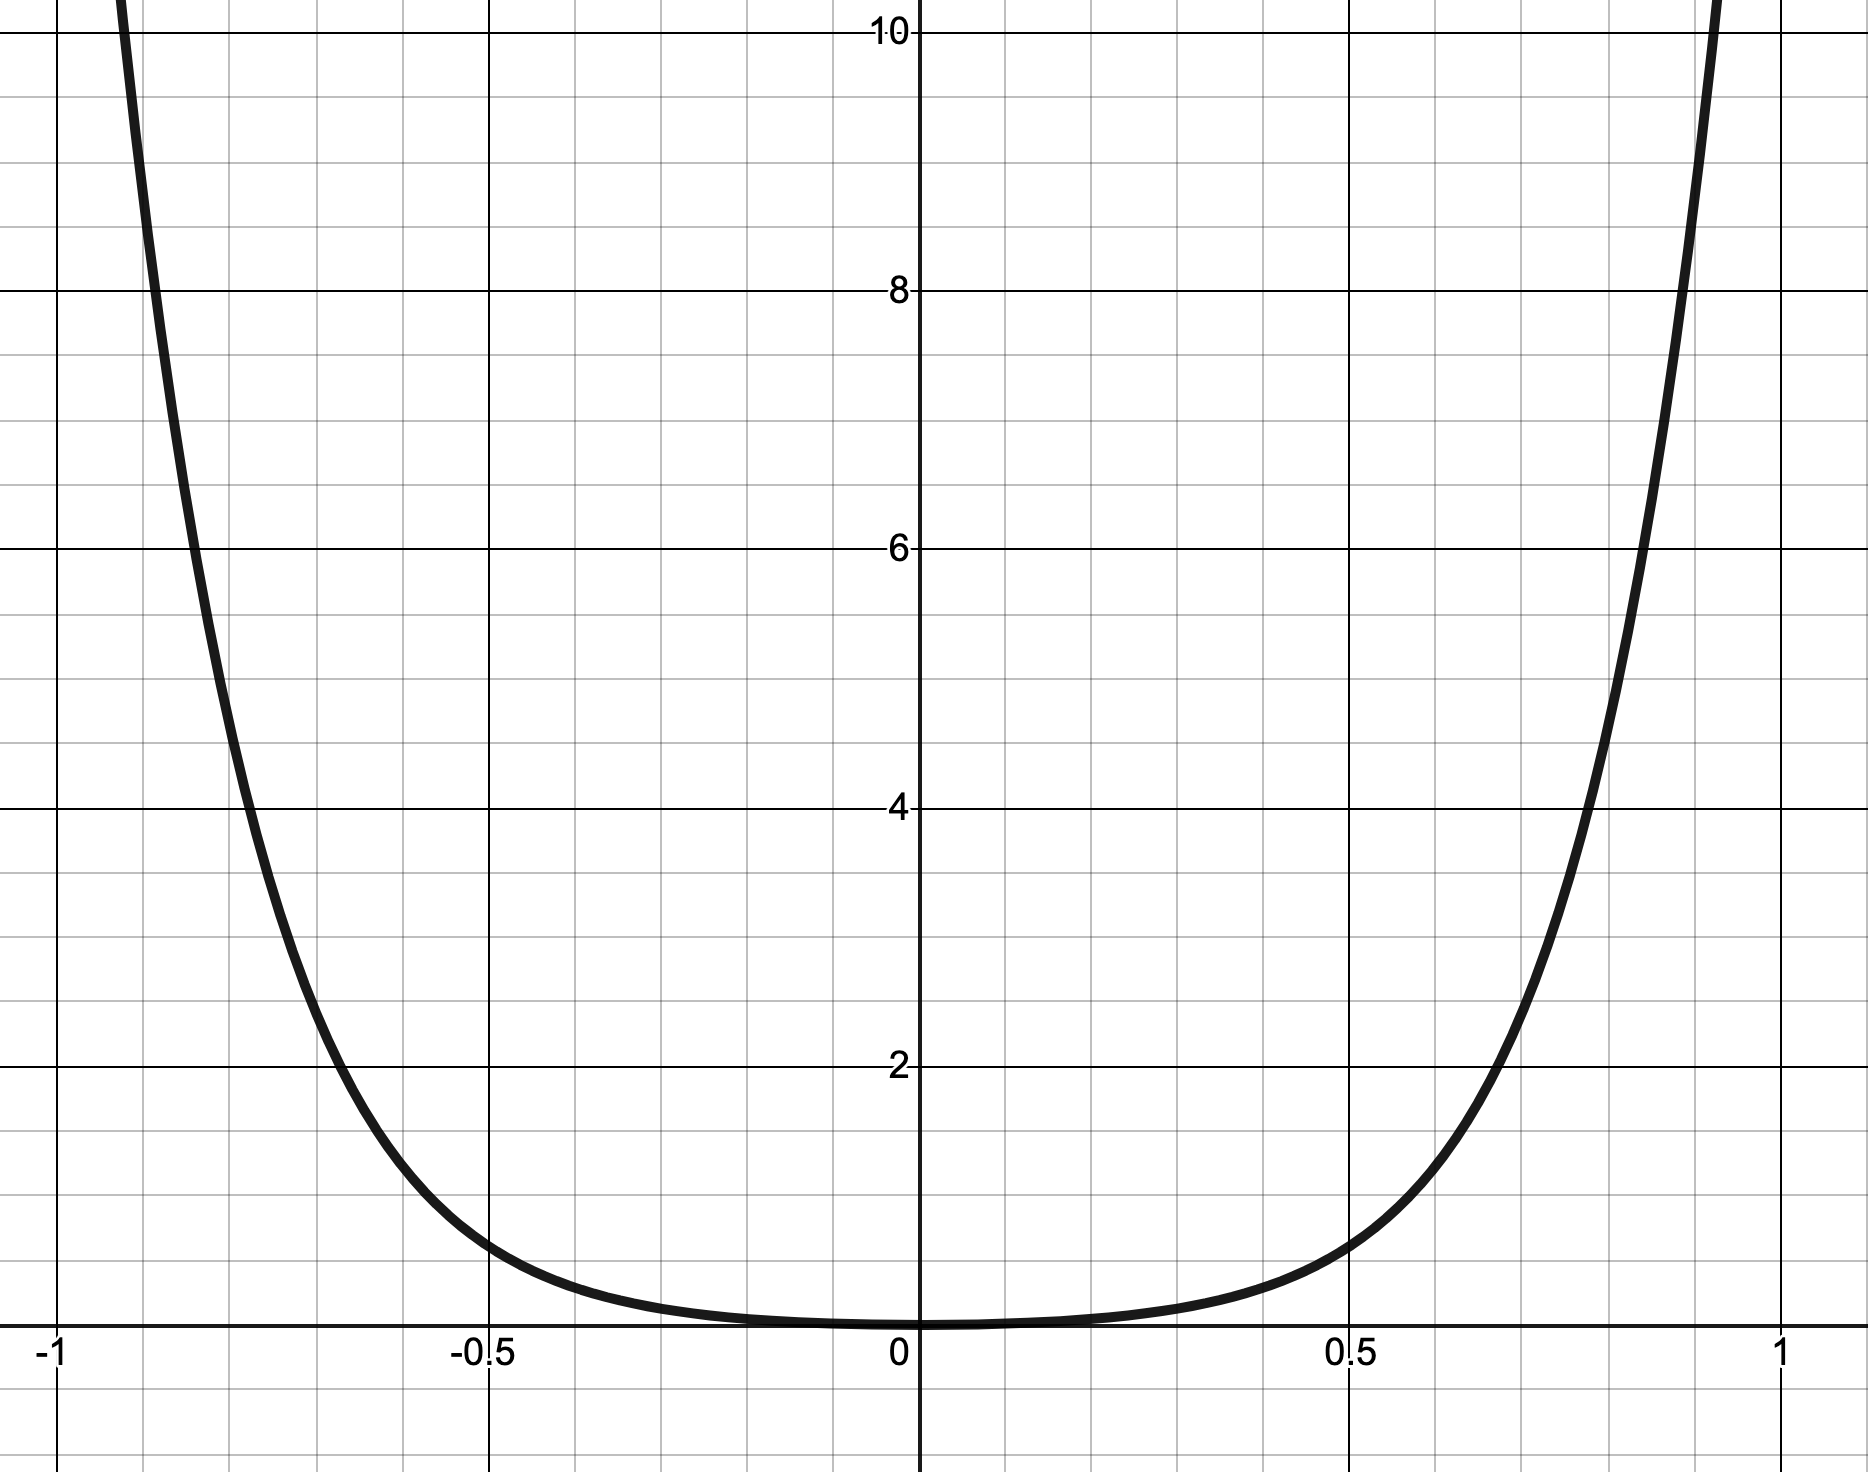
\includegraphics[scale=0.35]{images/productQuotient/11_1.png}
    \caption{}
    \end{figure}
    
    \begin{figure}[h!]
 \centering
    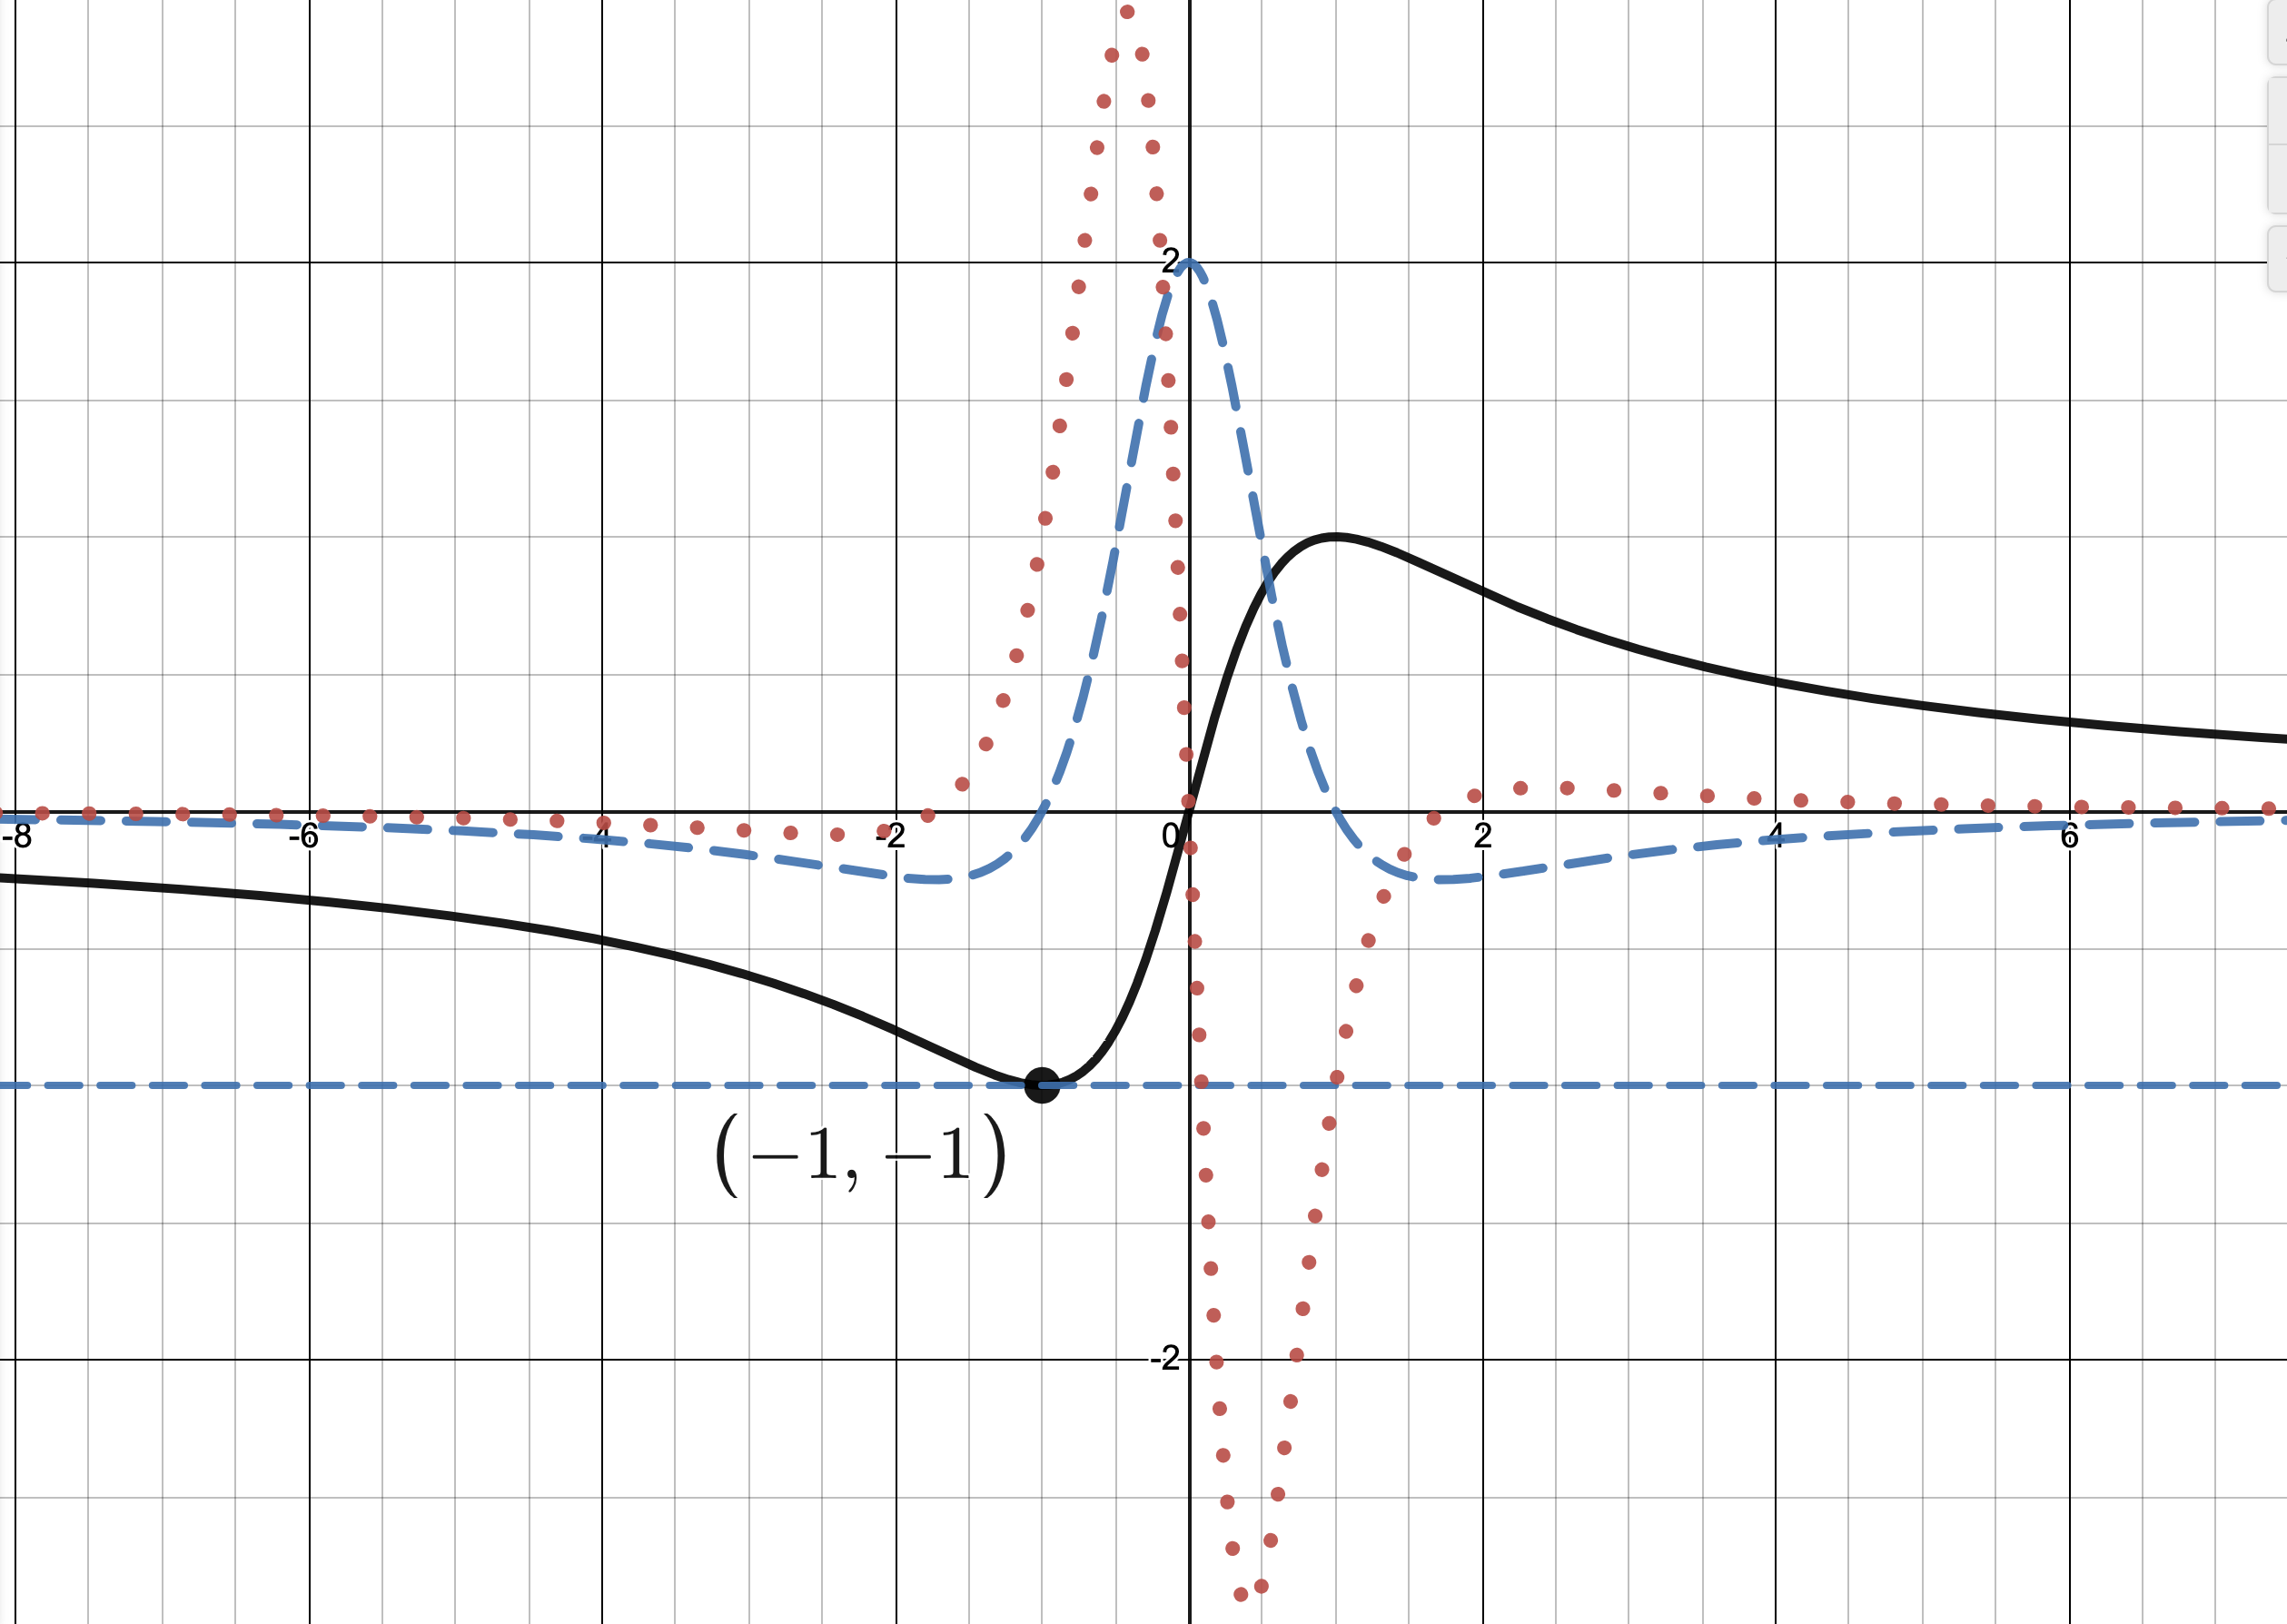
\includegraphics[scale=0.35]{images/productQuotient/11_2.png}
    \caption{}
    \end{figure}
\newpage
%%%%%%%%%%%%%%%%Dave's handout 3.1: Product and Quotient Rules %%%%%%%%%%
\subsection*{Combining Differentiation Rules}
%%%Examples%%%
\begin{example}
Given $f(x)=\left(\displaystyle\frac{2}{x+1}\right)^2$, find $f'(x)$ and identify any relative (local) maximum and relative (local) minimum points. A sign chart will help.
    %%short answer
    \begin{sol}
    \doublespacing{
    $f'(x)=\displaystyle\frac{-8}{(x+1)^3}$; No relative extreme points; Increasing on $(-\infty,1)$, decreasing on $(-1,\infty)$, but $x=-1$ is not in the domain of the function and therefor does not correspond to a relative (local) maximum point.}
    \end{sol}
    %%solution
    \begin{solL}
    Complete solution here.....
    
    \end{solL}
    
\end{example}
\vspace{\stretch{1}}
%%%%%%%%%%%%%%%%Dave's handout 3.1: Product and Quotient Rules %%%%%%%%%%
\begin{example}
Given $f(x)=\displaystyle\frac{x}{(x^2+1)^3}$, find $f'(x)$ and identify the intervals for which the function is increasing and the intervals for which the function is decreasing.
    %%short answer
    \begin{sol}
   $f'(x)=\displaystyle\frac{-5x^2+1}{(x^2+1)^4}$; increasing on: $\left(-\frac{\sqrt{5}}{5},\frac{\sqrt{5}}{5}\right)$; decreasing on: $\left(-\infty,-\frac{\sqrt{5}}{5}\right)\cup \left(\frac{\sqrt{5}}{5},\infty\right)$
    \end{sol}
    %%solution
    \begin{solL}
    Complete solution here.....
    
    \end{solL}
    
\end{example}
\vspace{\stretch{1}}
\newpage
 \begin{figure}[h!]
 \centering
    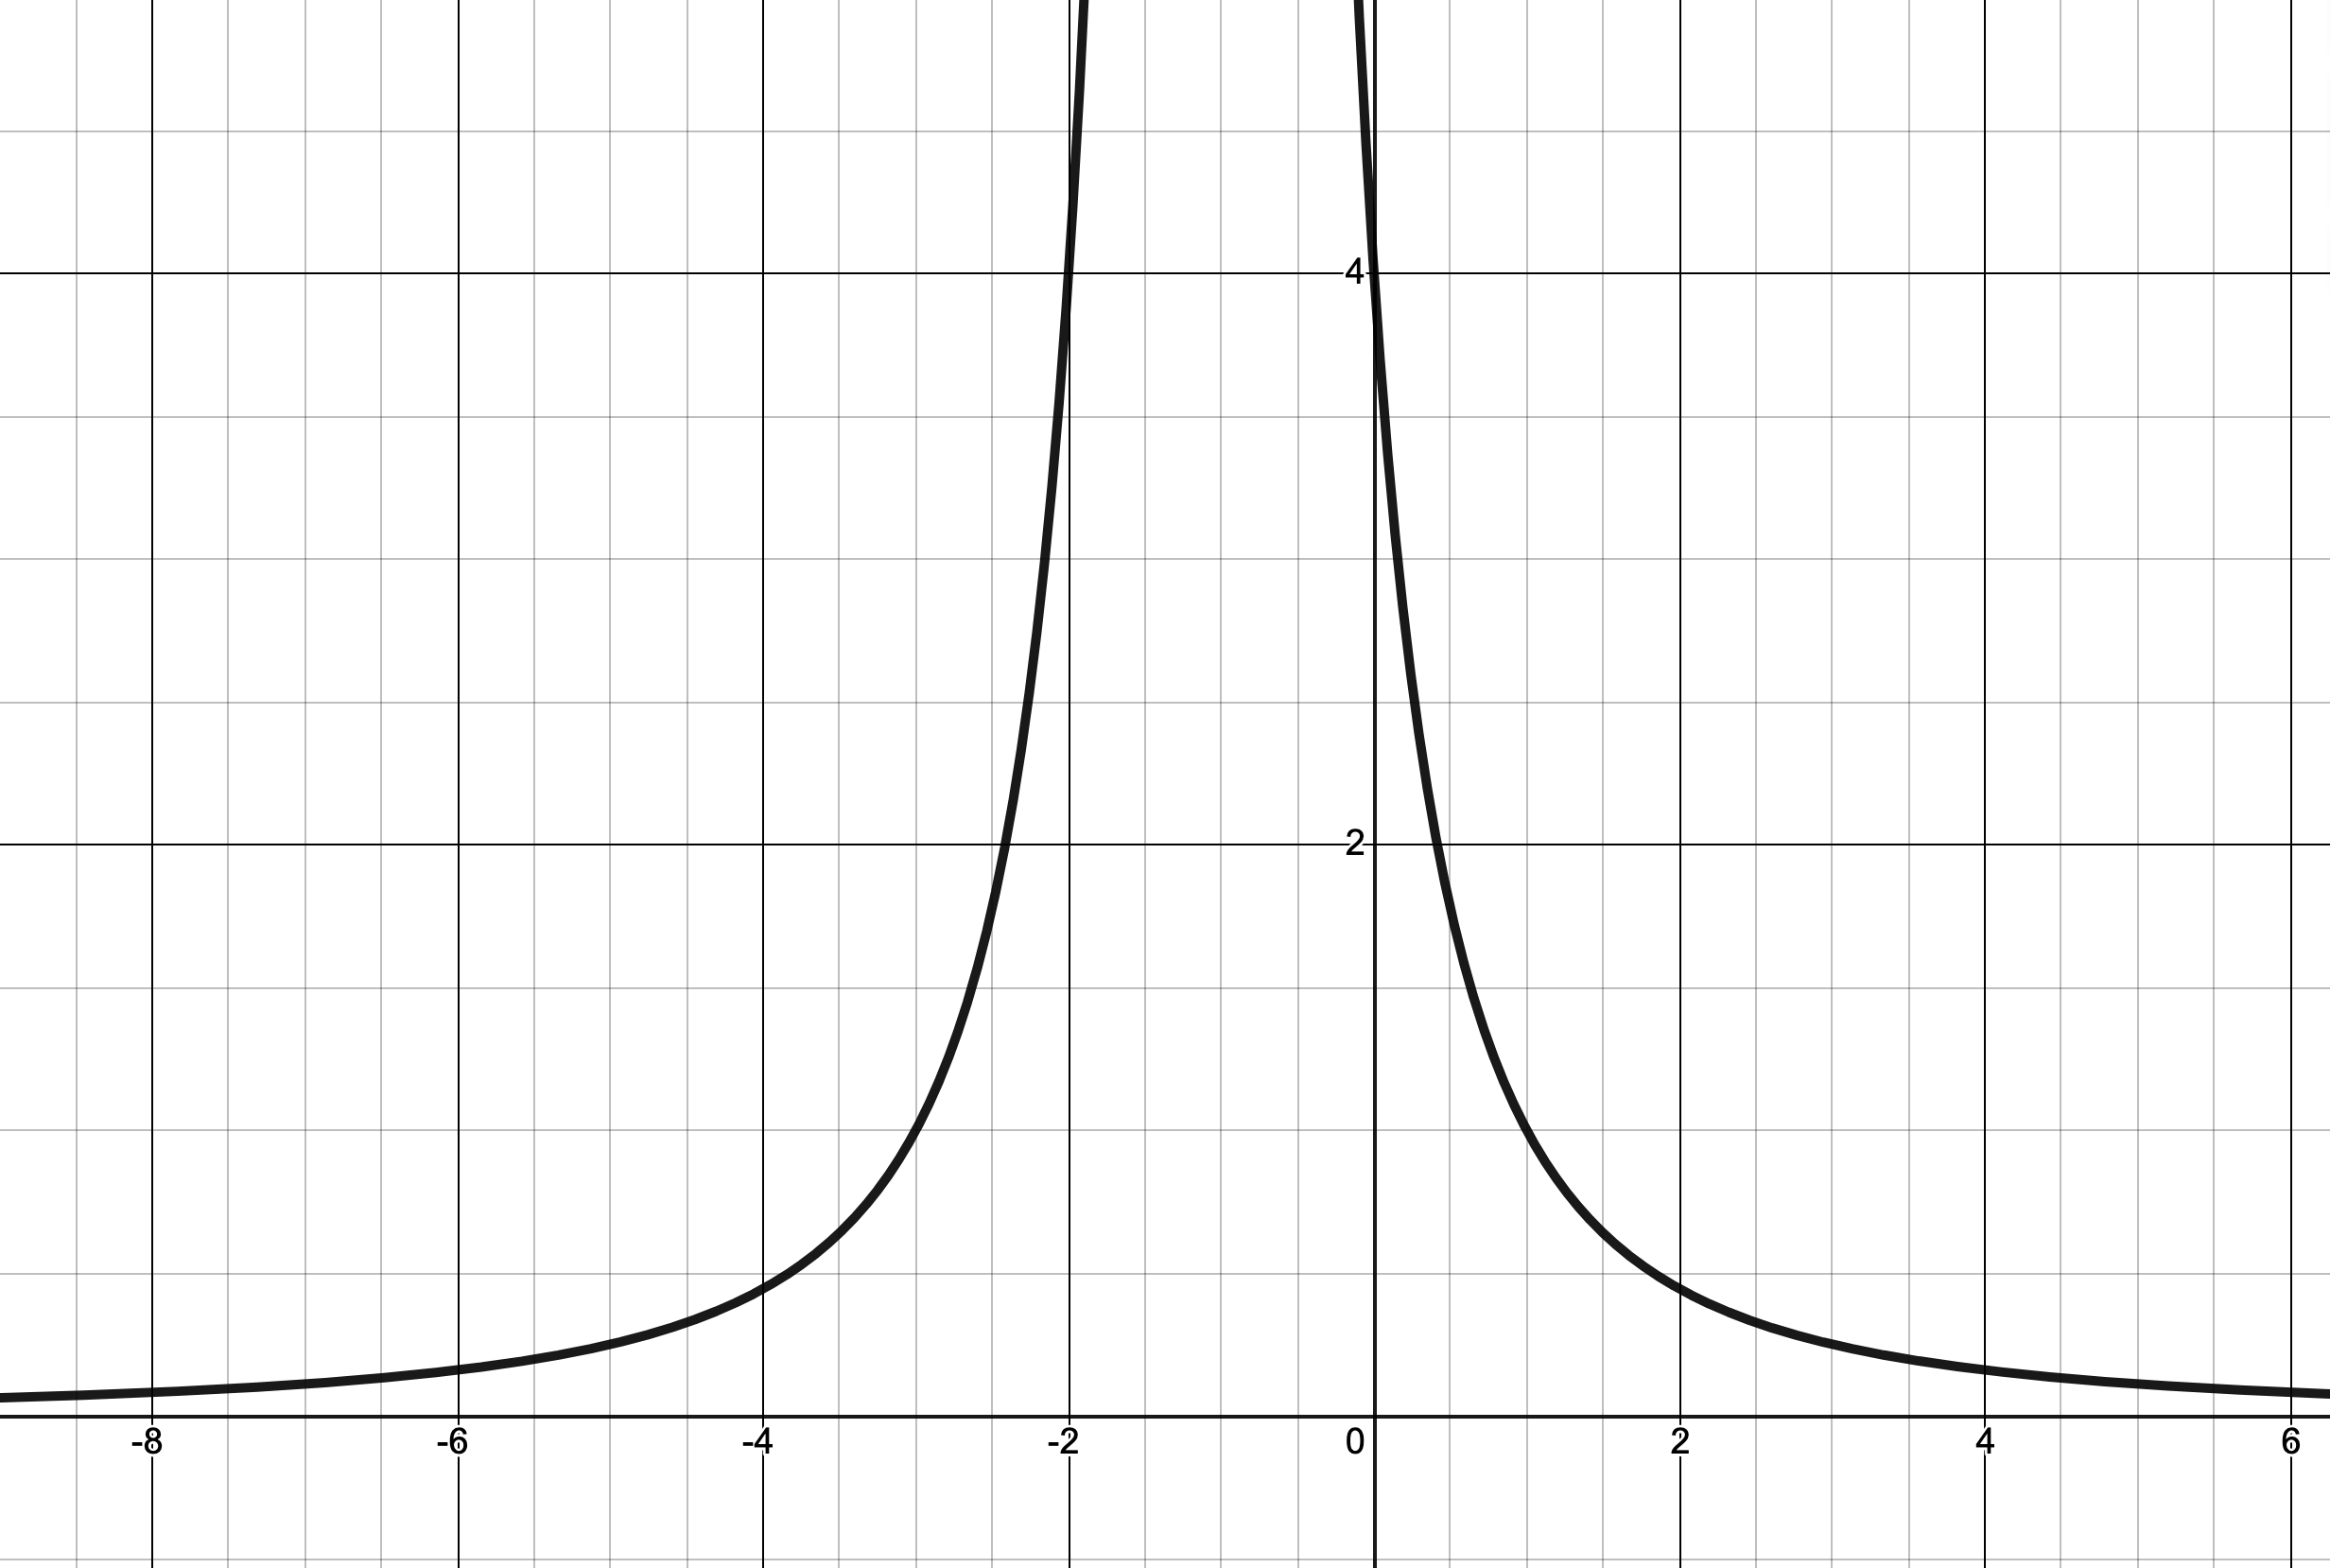
\includegraphics[scale=0.175]{images/productQuotient/11_3.png}
    \caption{}
    \end{figure}
    
    \begin{figure}[h!]
 \centering
    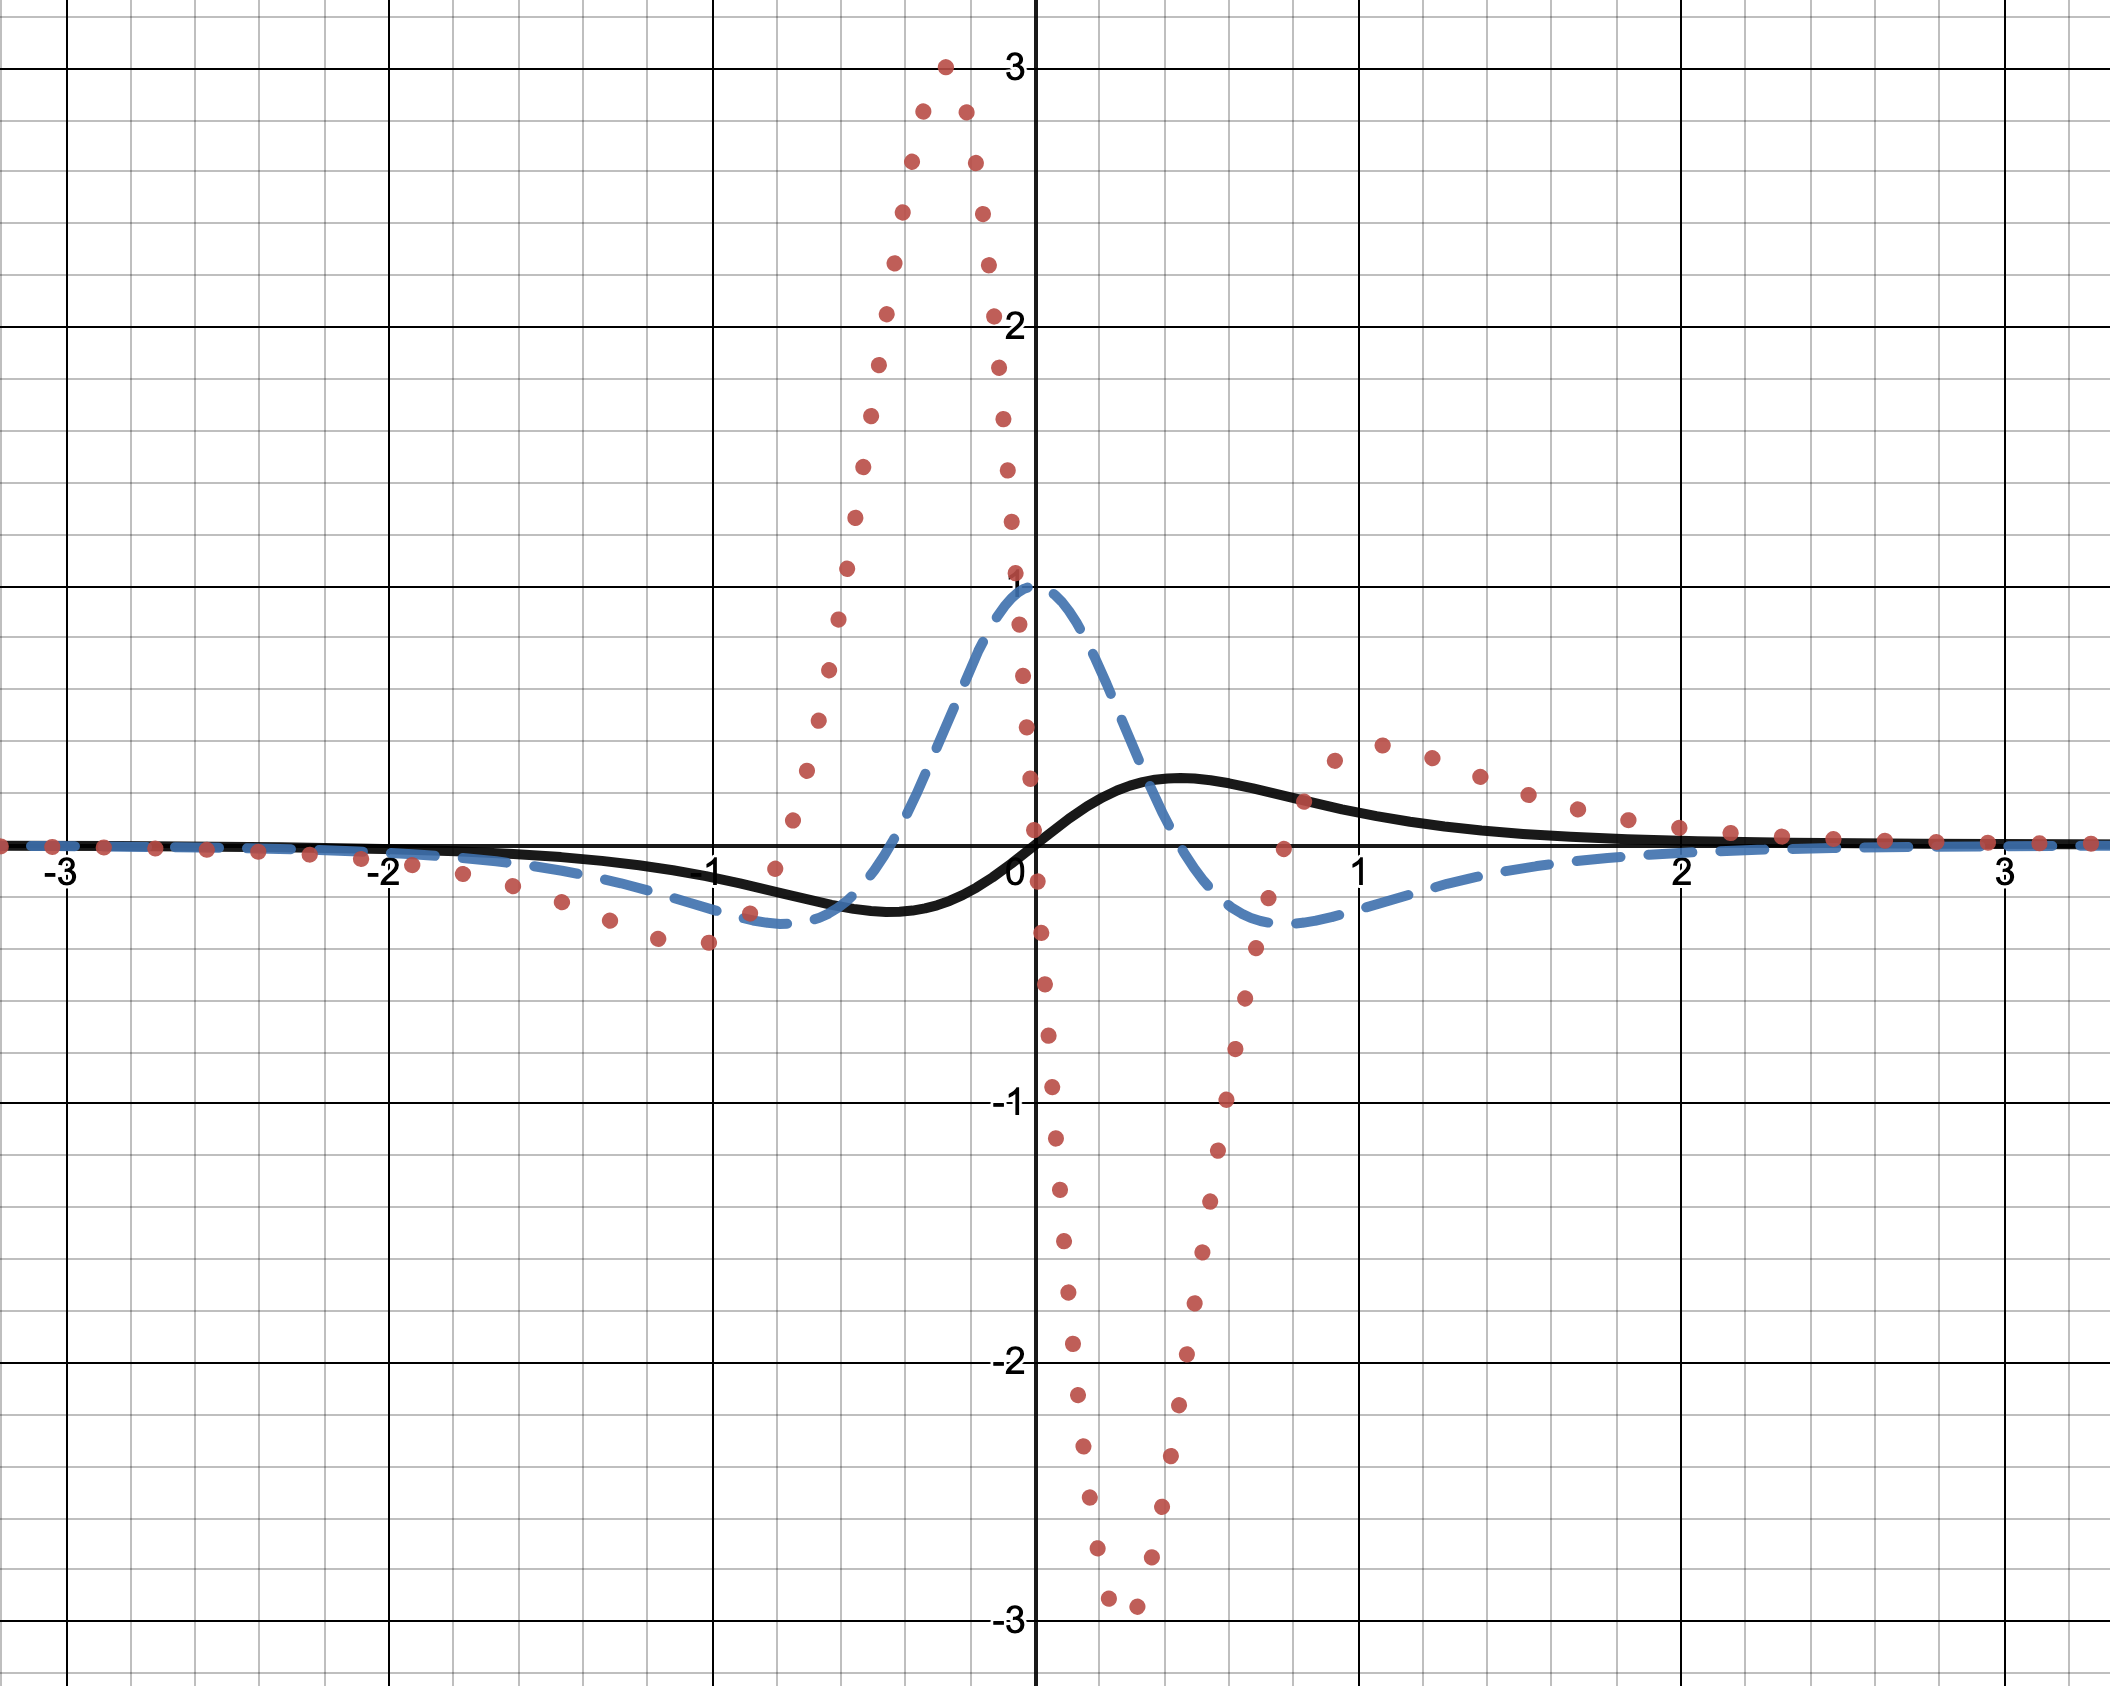
\includegraphics[scale=0.35]{images/productQuotient/11_4.png}
    \caption{}
    \end{figure}
%%%%%%%%%%%%%%%%Dave's handout 3.1: Quotient Rule Application%%%%%%%%%%
\subsection*{Quotient Rule Applications}
A note on mathematical modeling:  A mathematical function may be used to model a process in which one variable demonstrates a relationship with another variable.  In many applications, time is the \underline{independent variable}, and some other quantity, the \underline{dependent variable}, is viewed as a “function” of time.  Through observation of the process, it may be possible to identify a mathematical function that can be used to predict the value of the dependent variable from the value of the independent variable.  That is, we use the function to “model” the process.  In the following two examples, note that the function we use is chosen to fit the “data” one would observe in the process.  In this case, we are observing how the amount of a drug in a patient’s bloodstream changes over time.
\newpage
%%%%%%%%%%%%%%%%Dave's handout 3.1: Quotient Rule Application%%%%%%%%%%
\begin{example}
\underline{A Bolus Injection (“Shot”) of a Drug}(Note:  The drug will seep into the bloodstream and then it will be metabolized by the body.)  A patient is given an injection of a drug into a shoulder muscle and the following function is used to model the amount, $\bm{A}$ (in milligrams), of the drug in the patient’s bloodstream at time $\bm{t}$ hours after the injection:
\begin{equation*}
    A(t)=\frac{10t}{1+0.25t^2}\ mg.;\ t\ge 0
\end{equation*}
\renewcommand{\labelenumi}{(\alph{enumi})}
\begin{enumerate}[leftmargin=*]
    \item Determine the \textbf{time} at which the amount of the drug will be at its largest value. \vspace{\stretch{1}}
    \item Determine the maximum amount of the drug that will be in the bloodstream. \vspace{\stretch{1}}
    \item Determine the \textbf{rate} at which the amount of the drug in the bloodstream is changing at time $t=4$ hours.  Indicate if the amount is increasing or decreasing at this time, and include the units on the rate of change.\vspace{\stretch{1}}
\end{enumerate}
    %%short answer
    \begin{sol}
   \begin{enumInline1}
   \item $A'(t)=\displaystyle\frac{-2.5t^2+10}{(1+0.25t^2)^2}$; Relative ( and Absolute) max at $t=2$ hours 
   \item $A(2)=10$mg.  
   \item  $A'(4)=-1.2$ mg. per hour; decreasing at a rate 1.2 mg. per hour.
   \end{enumInline1}
    \end{sol}
    %%solution
    \begin{solL}
    Complete solution here.....
    
    \end{solL}
    
\end{example}
\newpage
 \begin{figure}[h!]
 \centering
    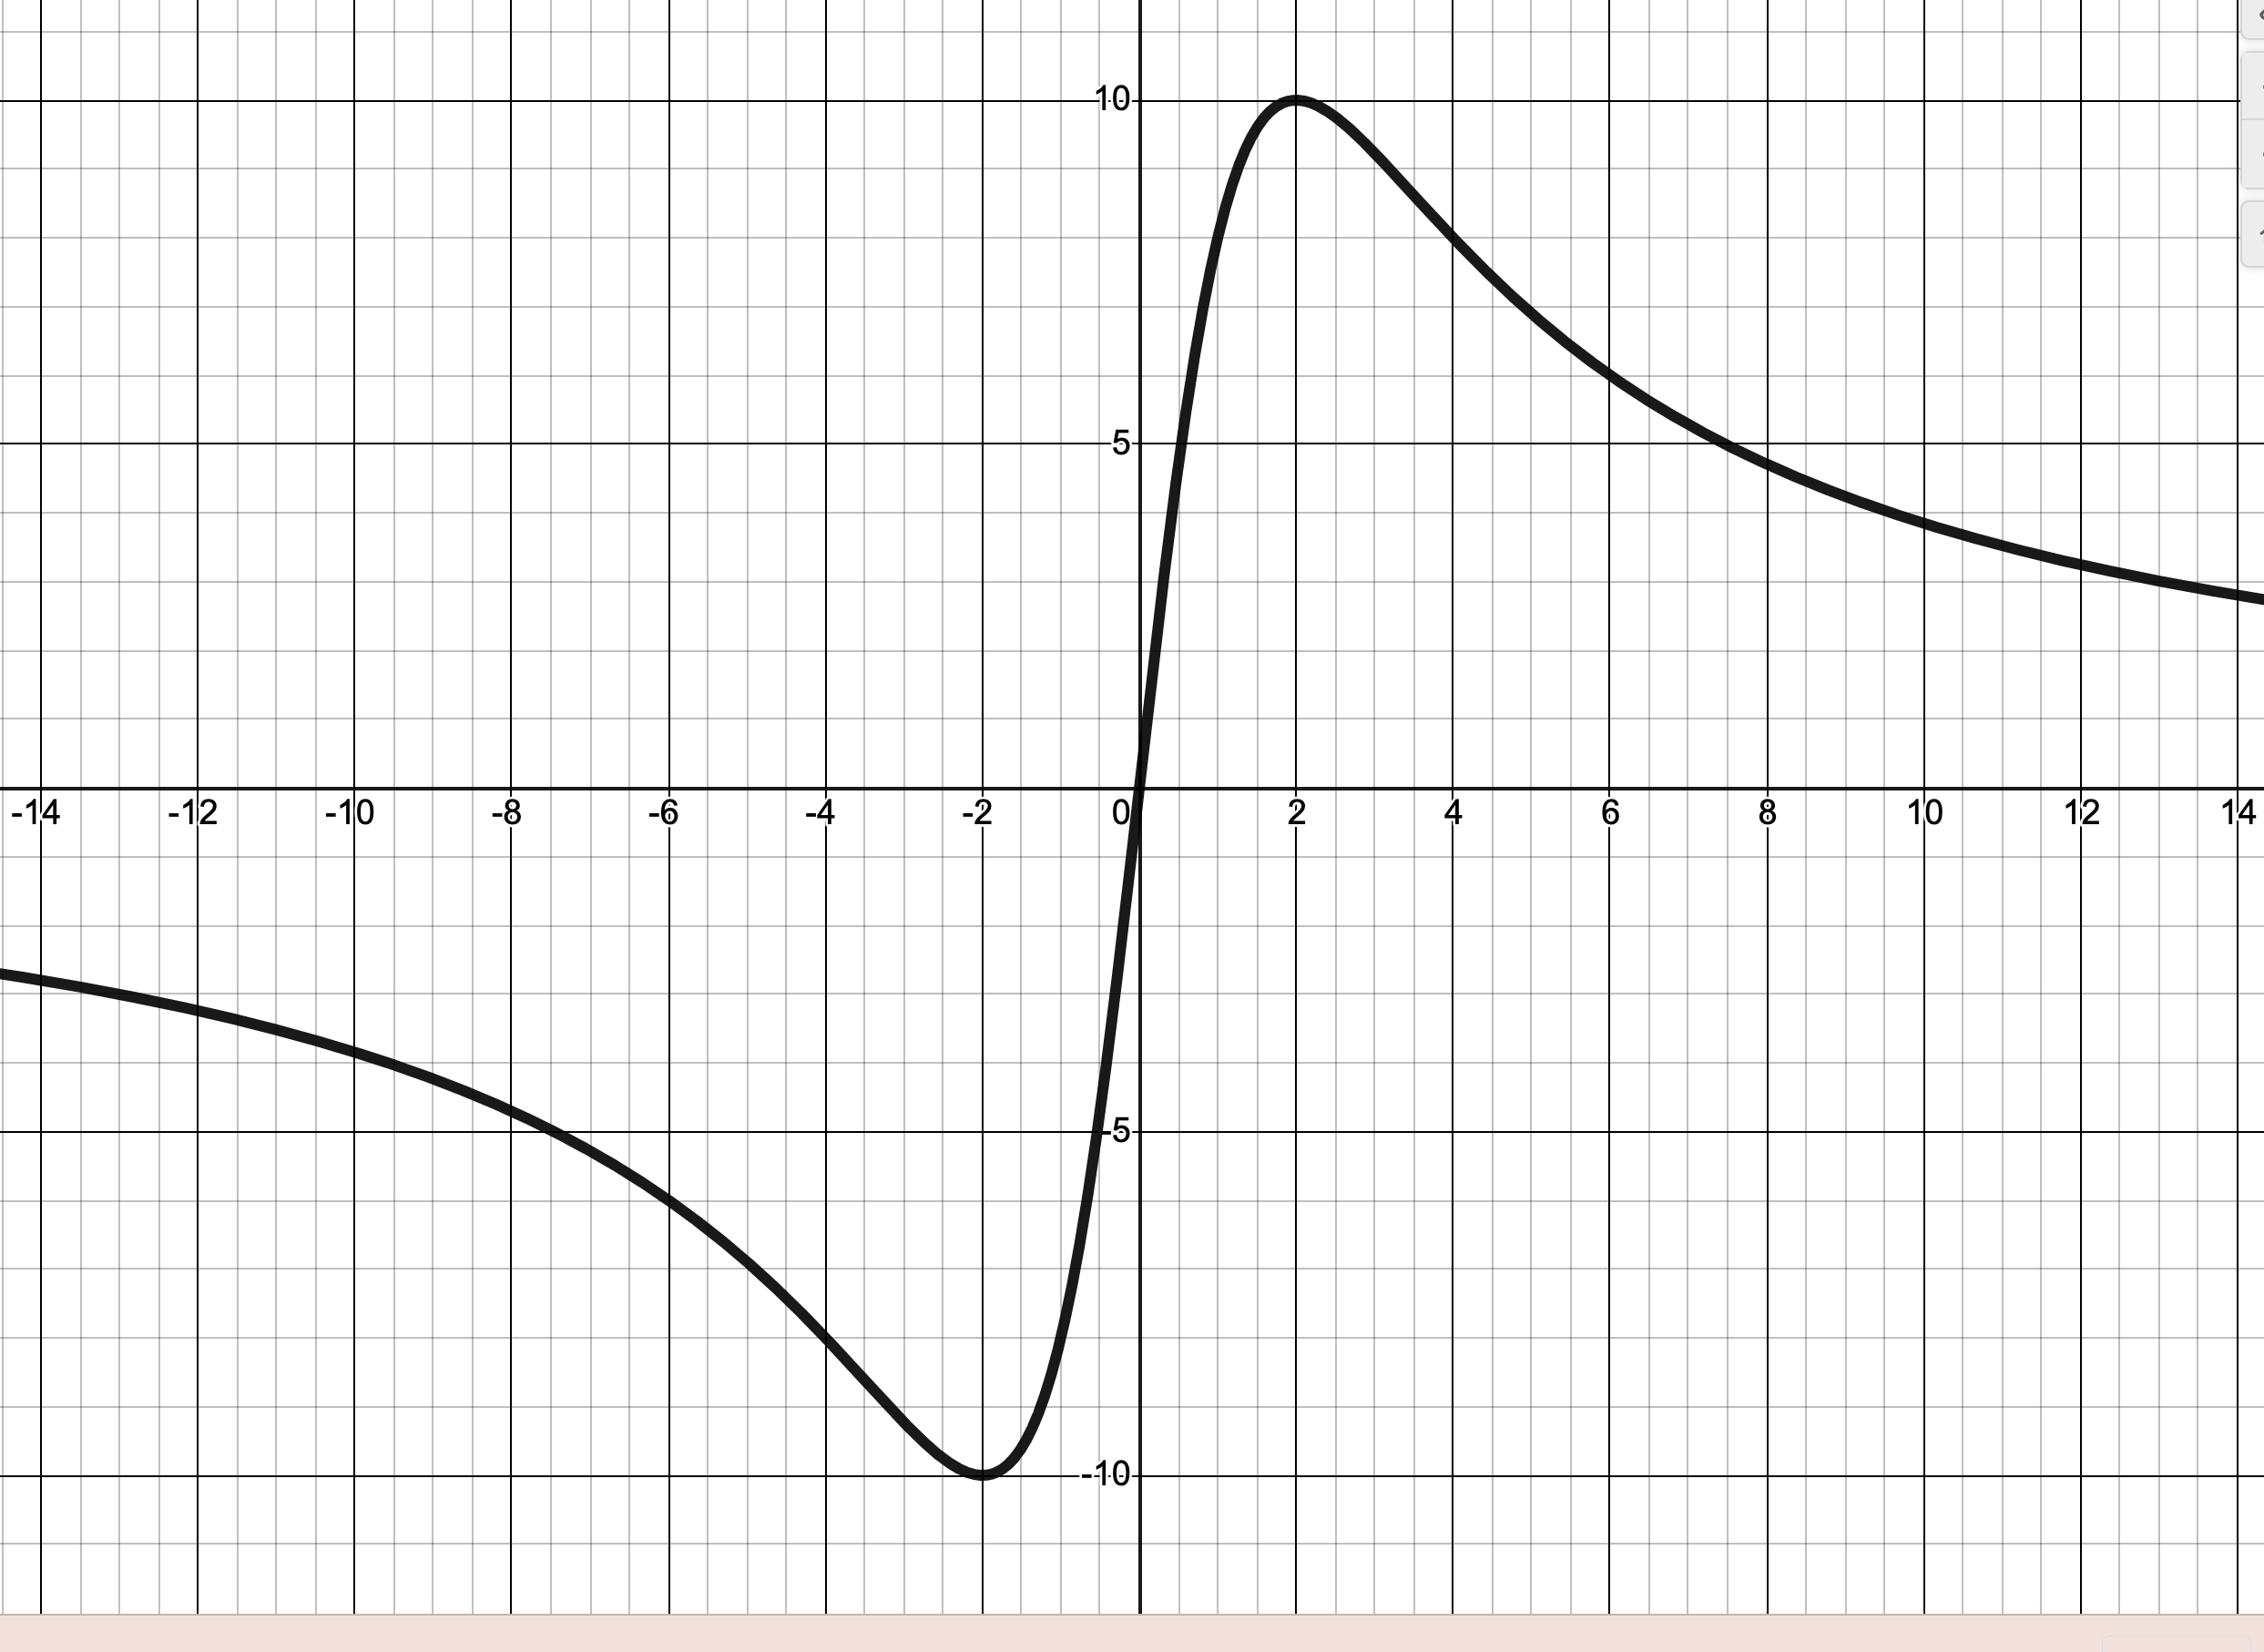
\includegraphics[scale=0.20]{images/productQuotient/11_5a.png}
    \caption{}
    \end{figure}
    
    \begin{figure}[h!]
 \centering
    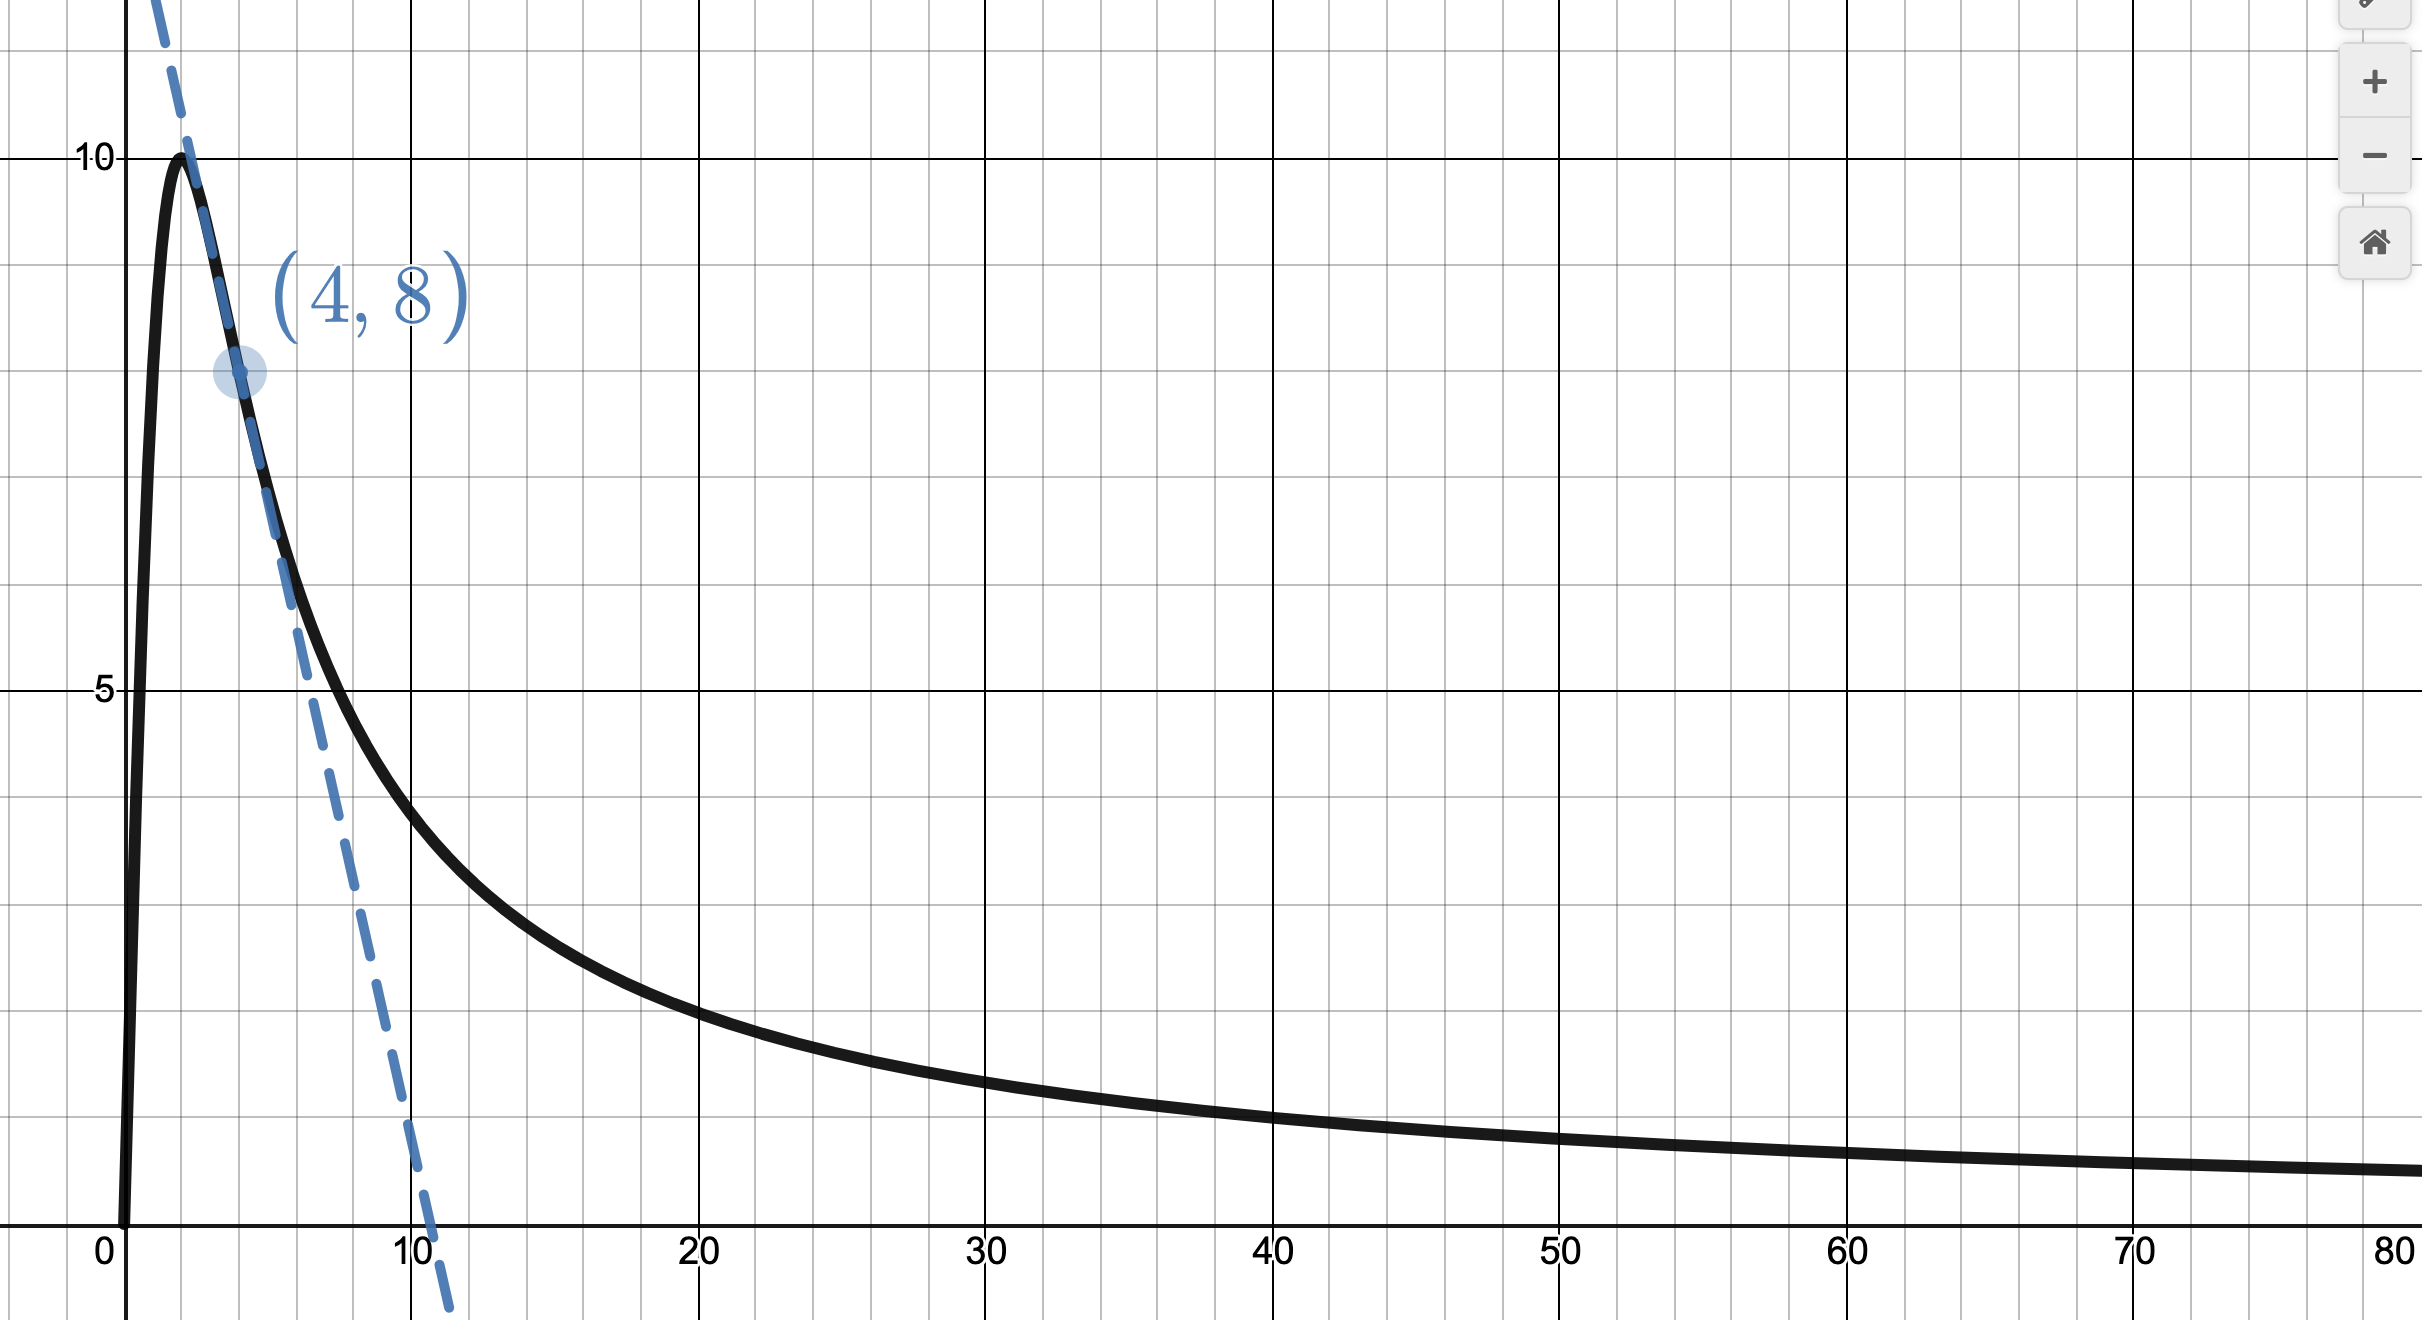
\includegraphics[scale=0.275]{images/productQuotient/11_5b.png}
    \caption{}
    \end{figure}
      \begin{figure}[h!]
 \centering
    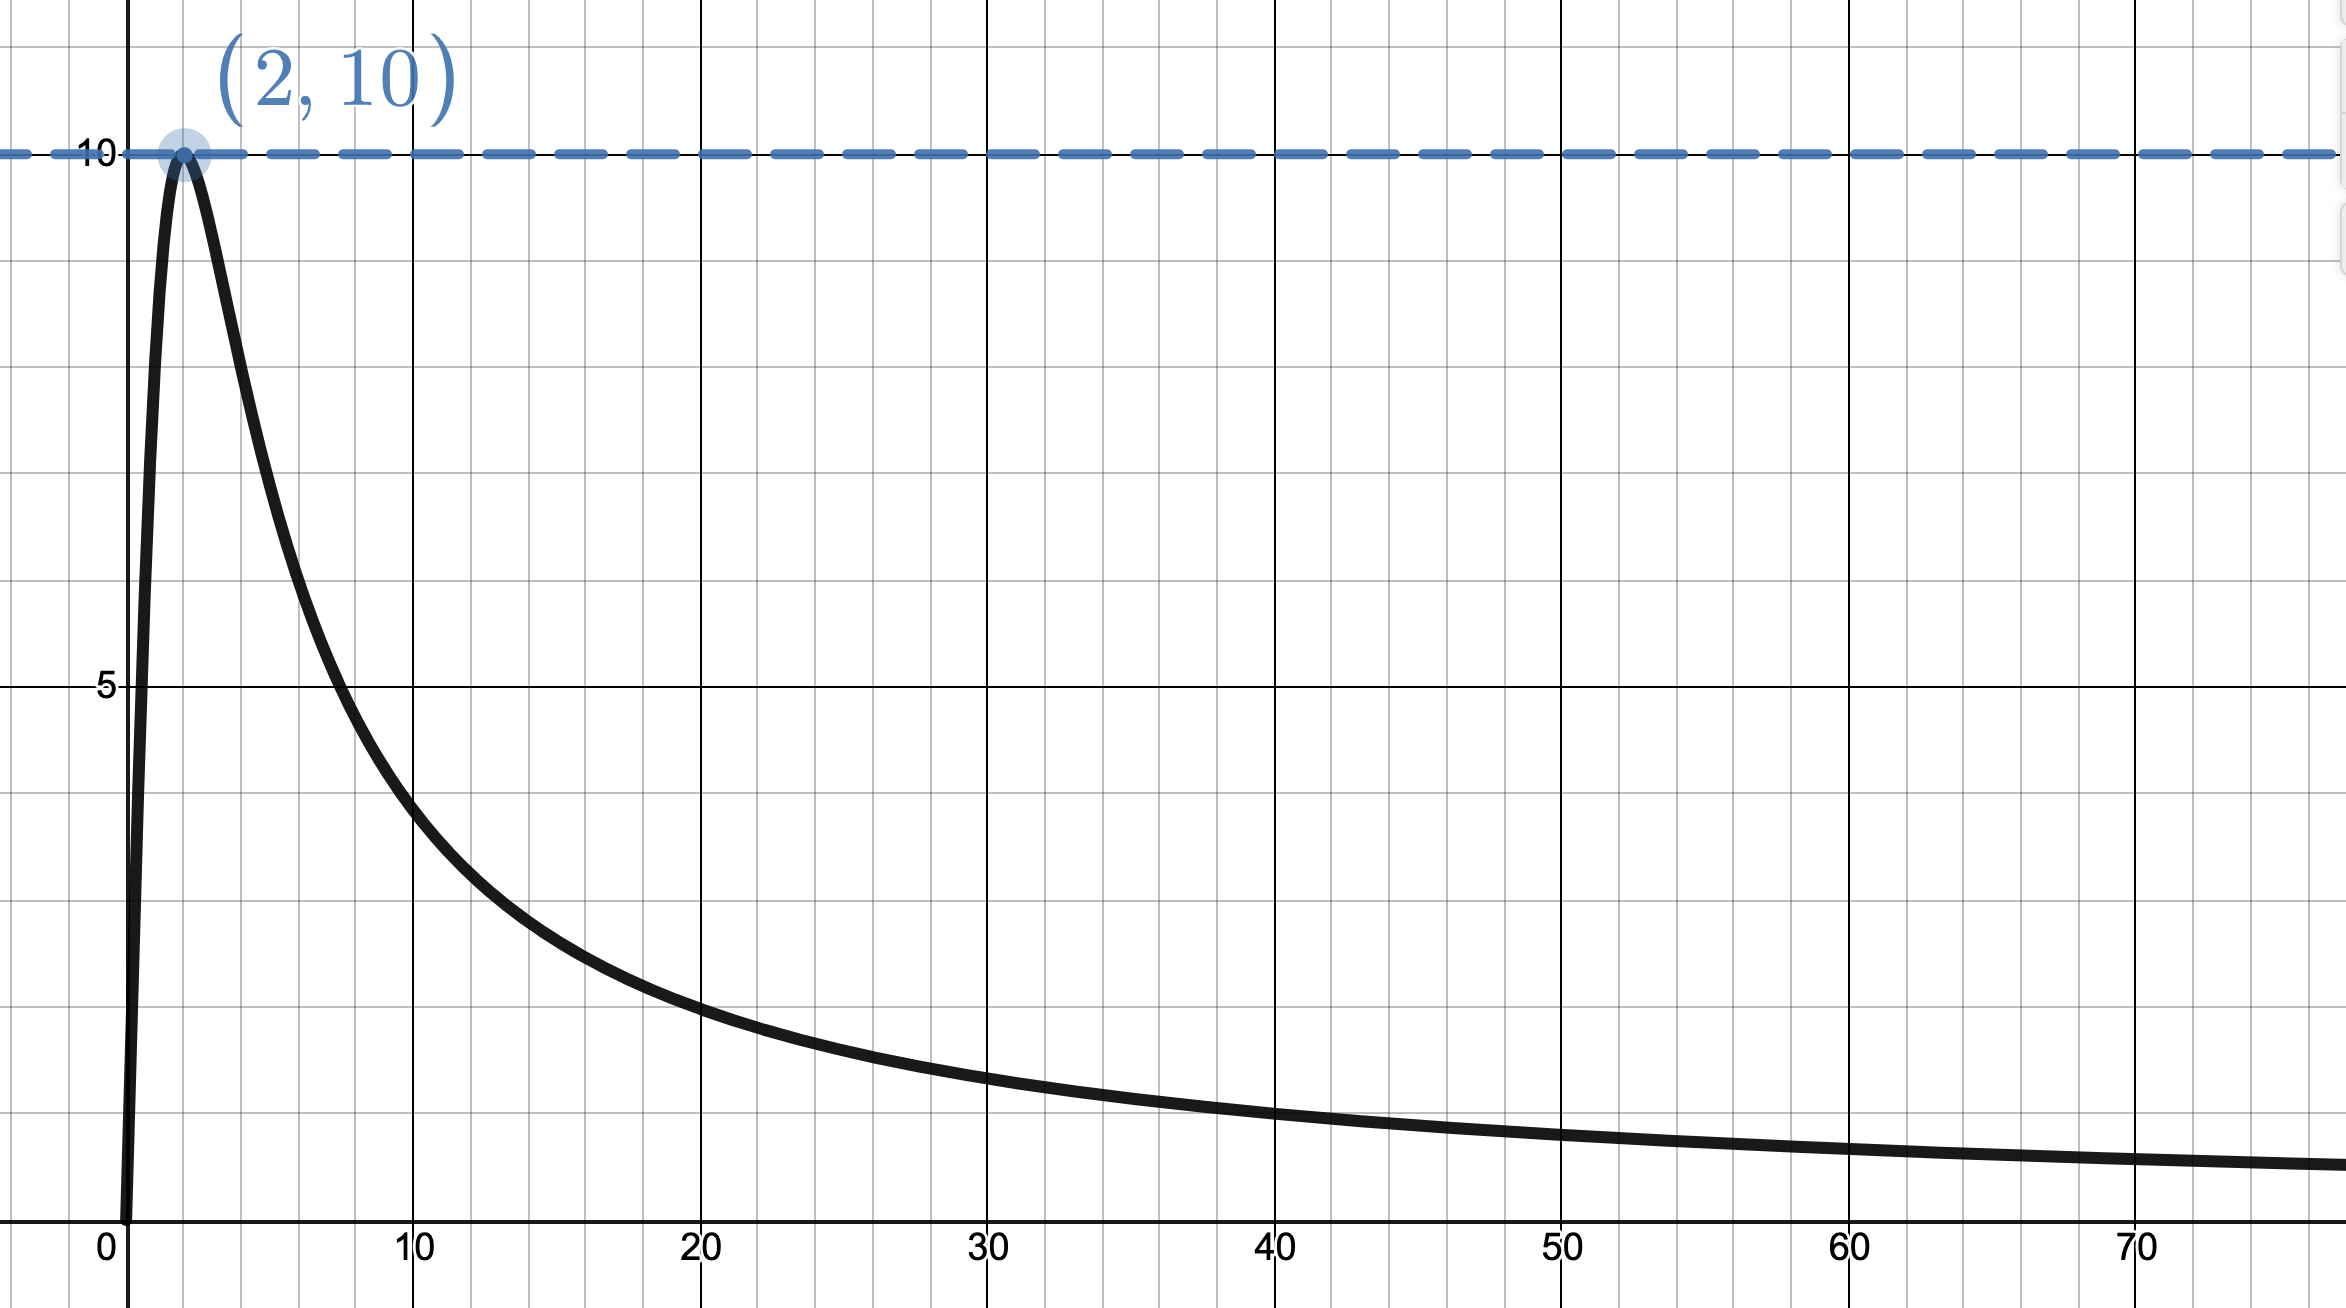
\includegraphics[scale=0.275]{images/productQuotient/11_5c.png}
    \caption{}
    \end{figure}
\newpage
%%%%%%%%%%%%%%%%Dave's handout 3.1: Quotient Rule Application%%%%%%%%%%
\begin{example}
\underline{A continuous intravenous injection of a drug} (Note:  The drug drips directly into a vein and at the same time the drug is being metabolized by the body.)  A patient is given an intravenous injection of a drug  and the following function is used to model the amount, $\bm{A}$ (in milligrams), of the drug in the patient’s bloodstream at time $\bm{t}$ hours after the injection::
\begin{equation*}
    A(t)=\frac{50t}{t+1}\ mg.;\ t\ge 0
\end{equation*}
\renewcommand{\labelenumi}{(\alph{enumi})}
\begin{enumerate}[leftmargin=*]
    \item 	Compare the rates of change of the drug at times $t=1$ hour and $t=4$ hours.  What do you notice?\vspace{\stretch{1}}
    \item According to this function, will the amount of the drug in the bloodstream ever reach a maximum value?  Use the derivative of the function to explain why or why not. \vspace{\stretch{1}}
\end{enumerate}
    %%short answer
    \begin{sol}
    %\renewcommand{\labelenumi}{\textbf{(\alph{enumi})}}
    \doublespacing{
   \begin{enumInline1}
   \item $A'(t)=\displaystyle\frac{50}{(t+1)^2}$; $A'(1)=12.5$ mg. per hour ; $A'(4)=2$ mg. per hour; The amount is increasing at both times, but it is increasing more rapidly at time $t=1$ hour.
   \item No. Note that $A'(t)>0$ for all values of $t$, so \underline{$A(t)$ is increasing} on $(0,\infty)$. However, $\lim\limits_{t \to \infty} A(t)=\lim\limits_{t \to \infty} \displaystyle\frac{50t}{t+1}=50$ mg. As such, the amount is NOT increasing without bound (horizontal asymptote) consistent with this observation is $\lim\limits_{t \to \infty} \displaystyle\frac{50}{(t+1)^2}=0$. The rate of graph is diminishing over time (the graph is becoming flatter).
%%%%%%%%%%%%%%%%%%%%%%%%%%%%%%%%%%%%%%%
  

    \end{enumInline1}}
 \begin{figure}[h]
 \centering
    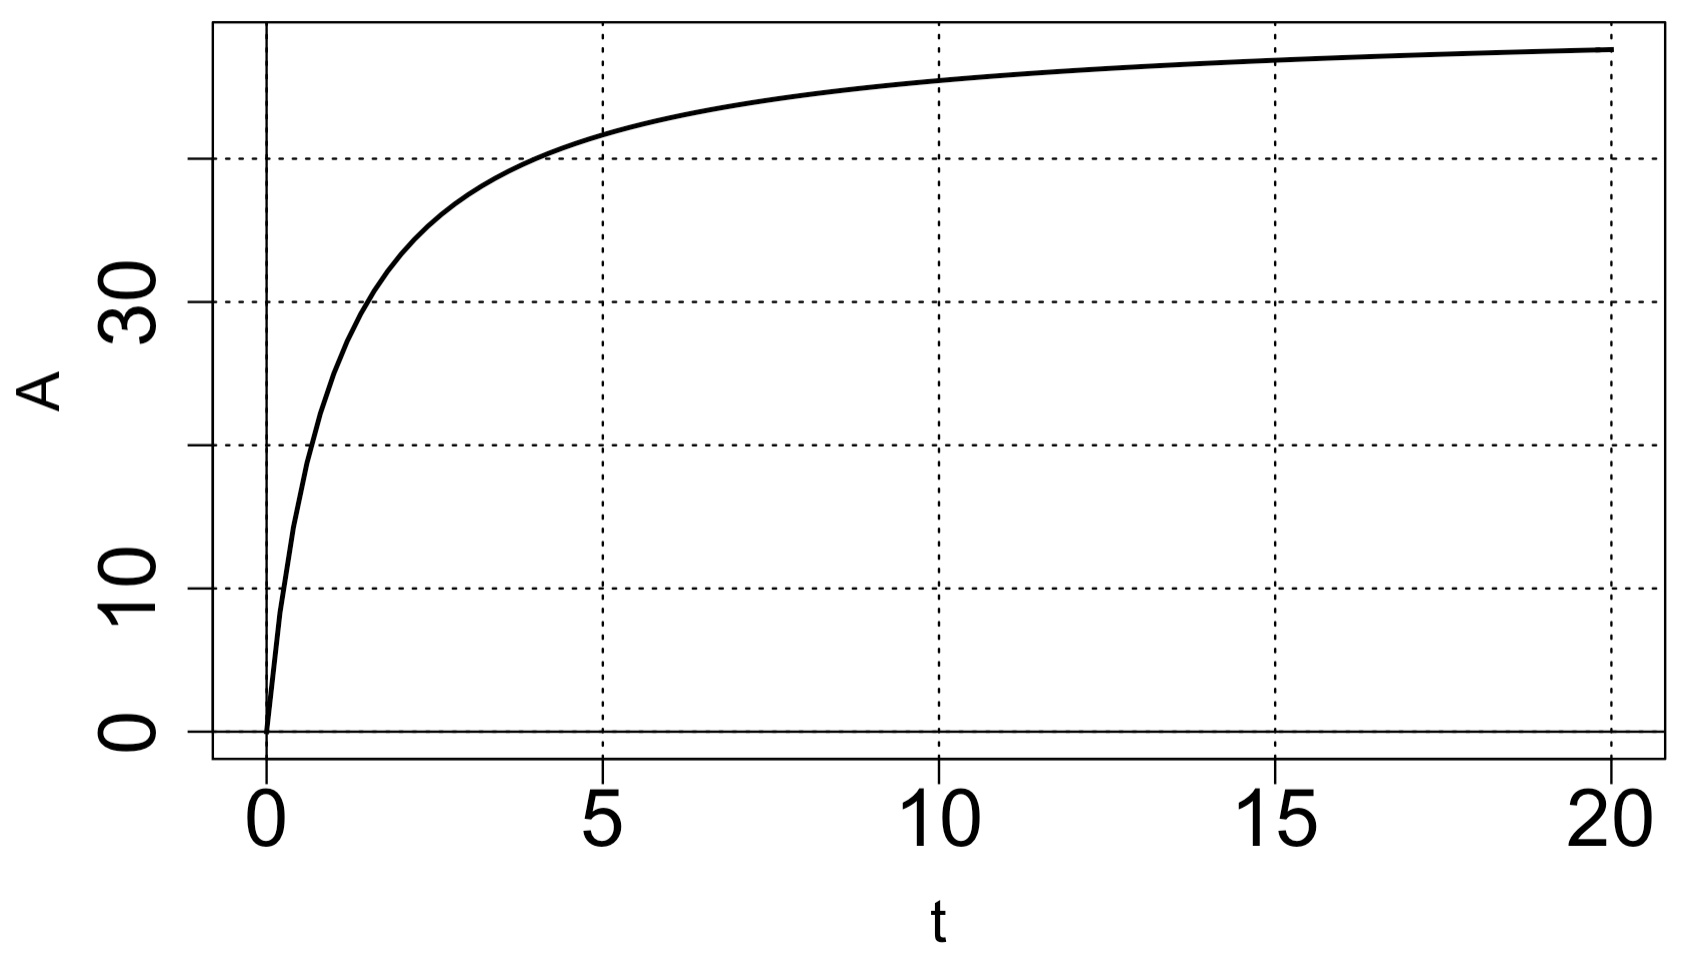
\includegraphics[width=0.4\textwidth]{images/productQuotient/Afunction.png}
    \caption{The graph of $A(t)$}
    \label{fig:Afunction}
    \end{figure}
    
    \begin{figure}[h]
 \centering
    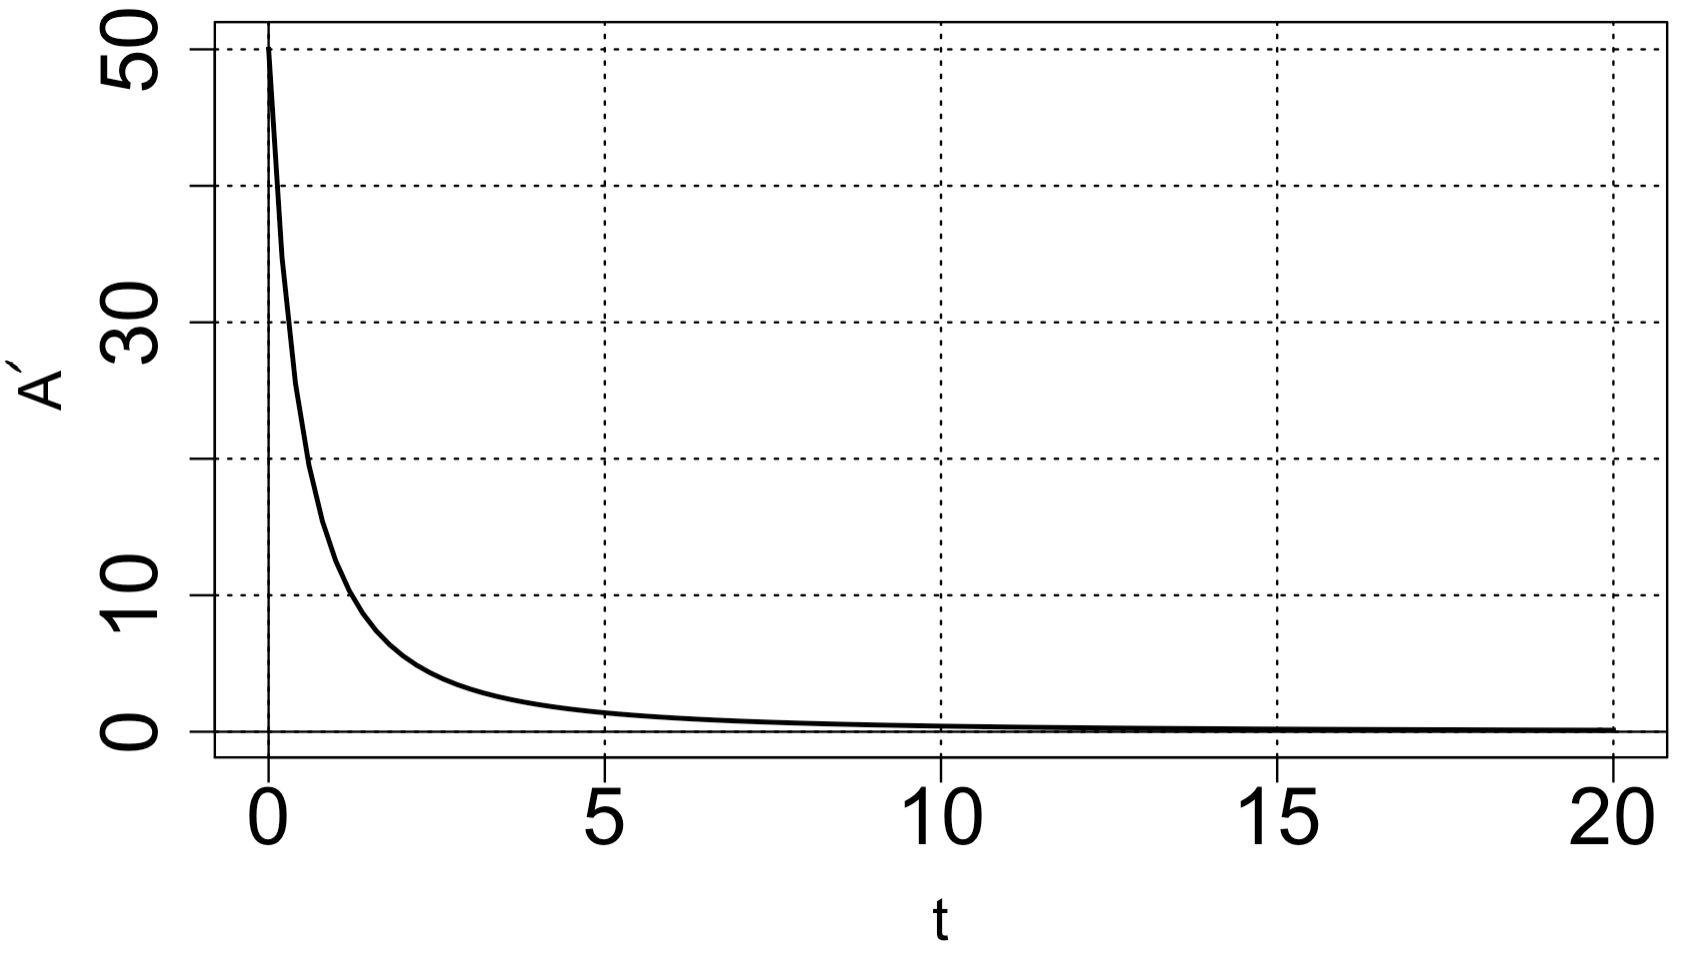
\includegraphics[width=0.4\textwidth]{images/productQuotient/AprimeFunction.png}
    \caption{The graph of $A'(t)$}
    \label{fig:AprimeFunction}
    \end{figure}
    \end{sol}
    %%solution
    \begin{solL}
    Complete solution here.....
    
    \end{solL}
    
\end{example}
\newpage
 \begin{figure}[h!]
 \centering
    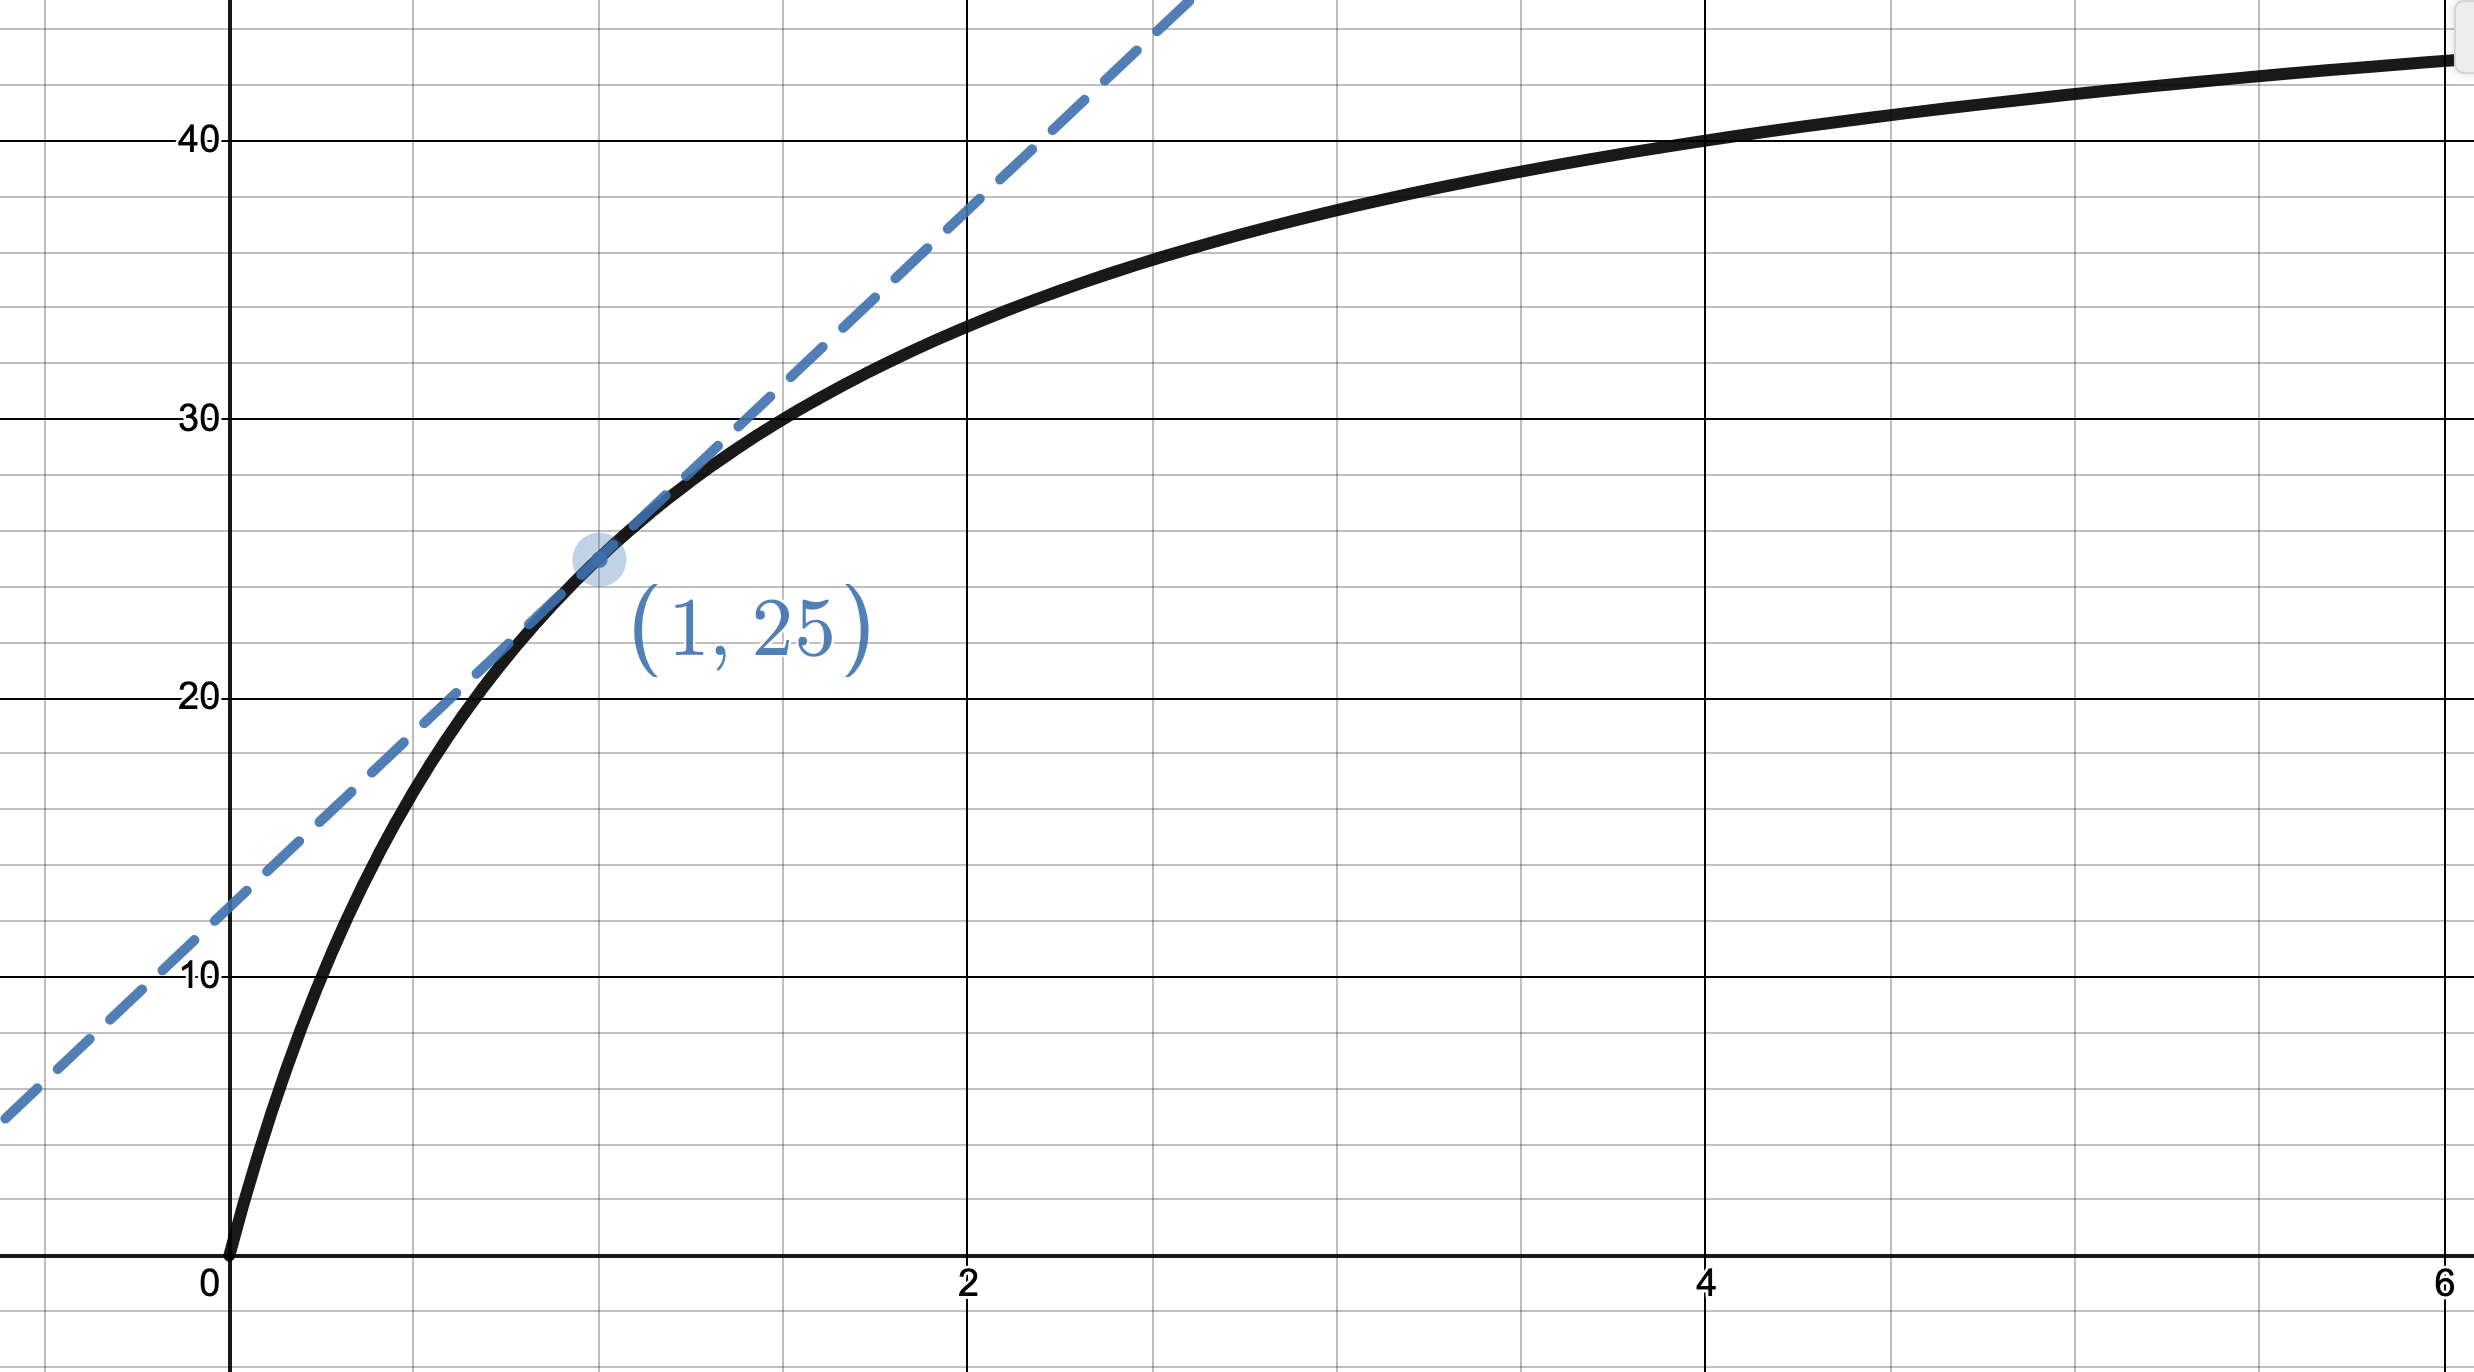
\includegraphics[scale=0.225]{images/productQuotient/11_6a.png}
    \caption{}
    \end{figure}
    
    \begin{figure}[h!]
 \centering
    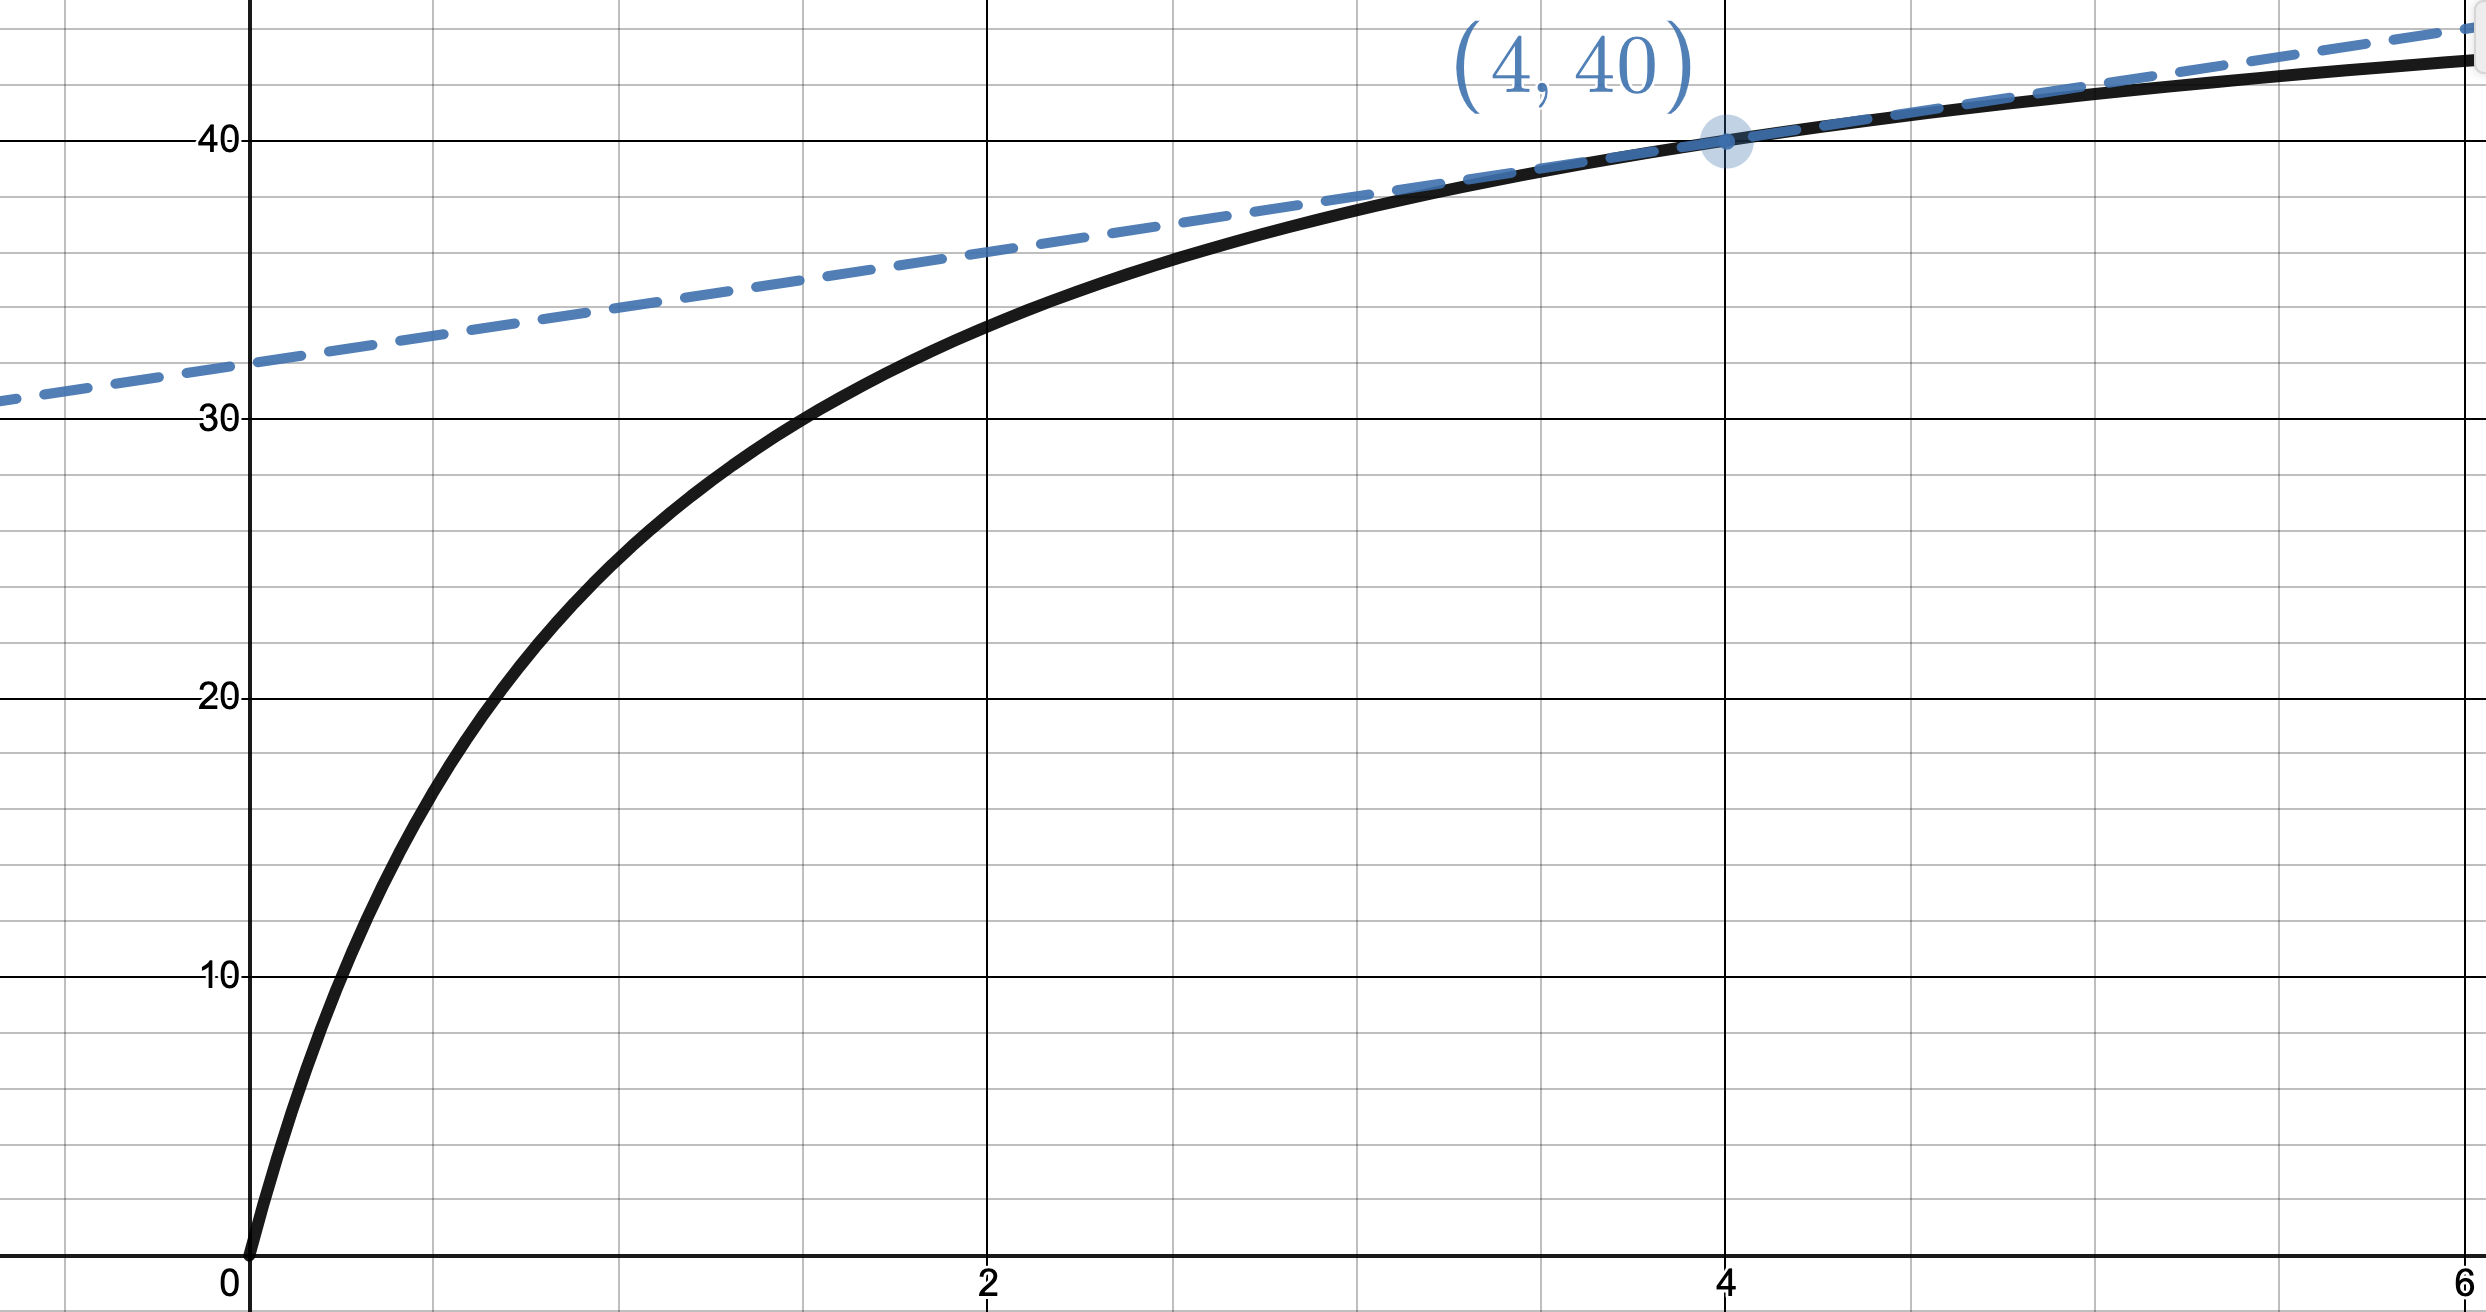
\includegraphics[scale=0.275]{images/productQuotient/11_6b.png}
    \caption{}
    \end{figure}
      \begin{figure}[h!]
 \centering
    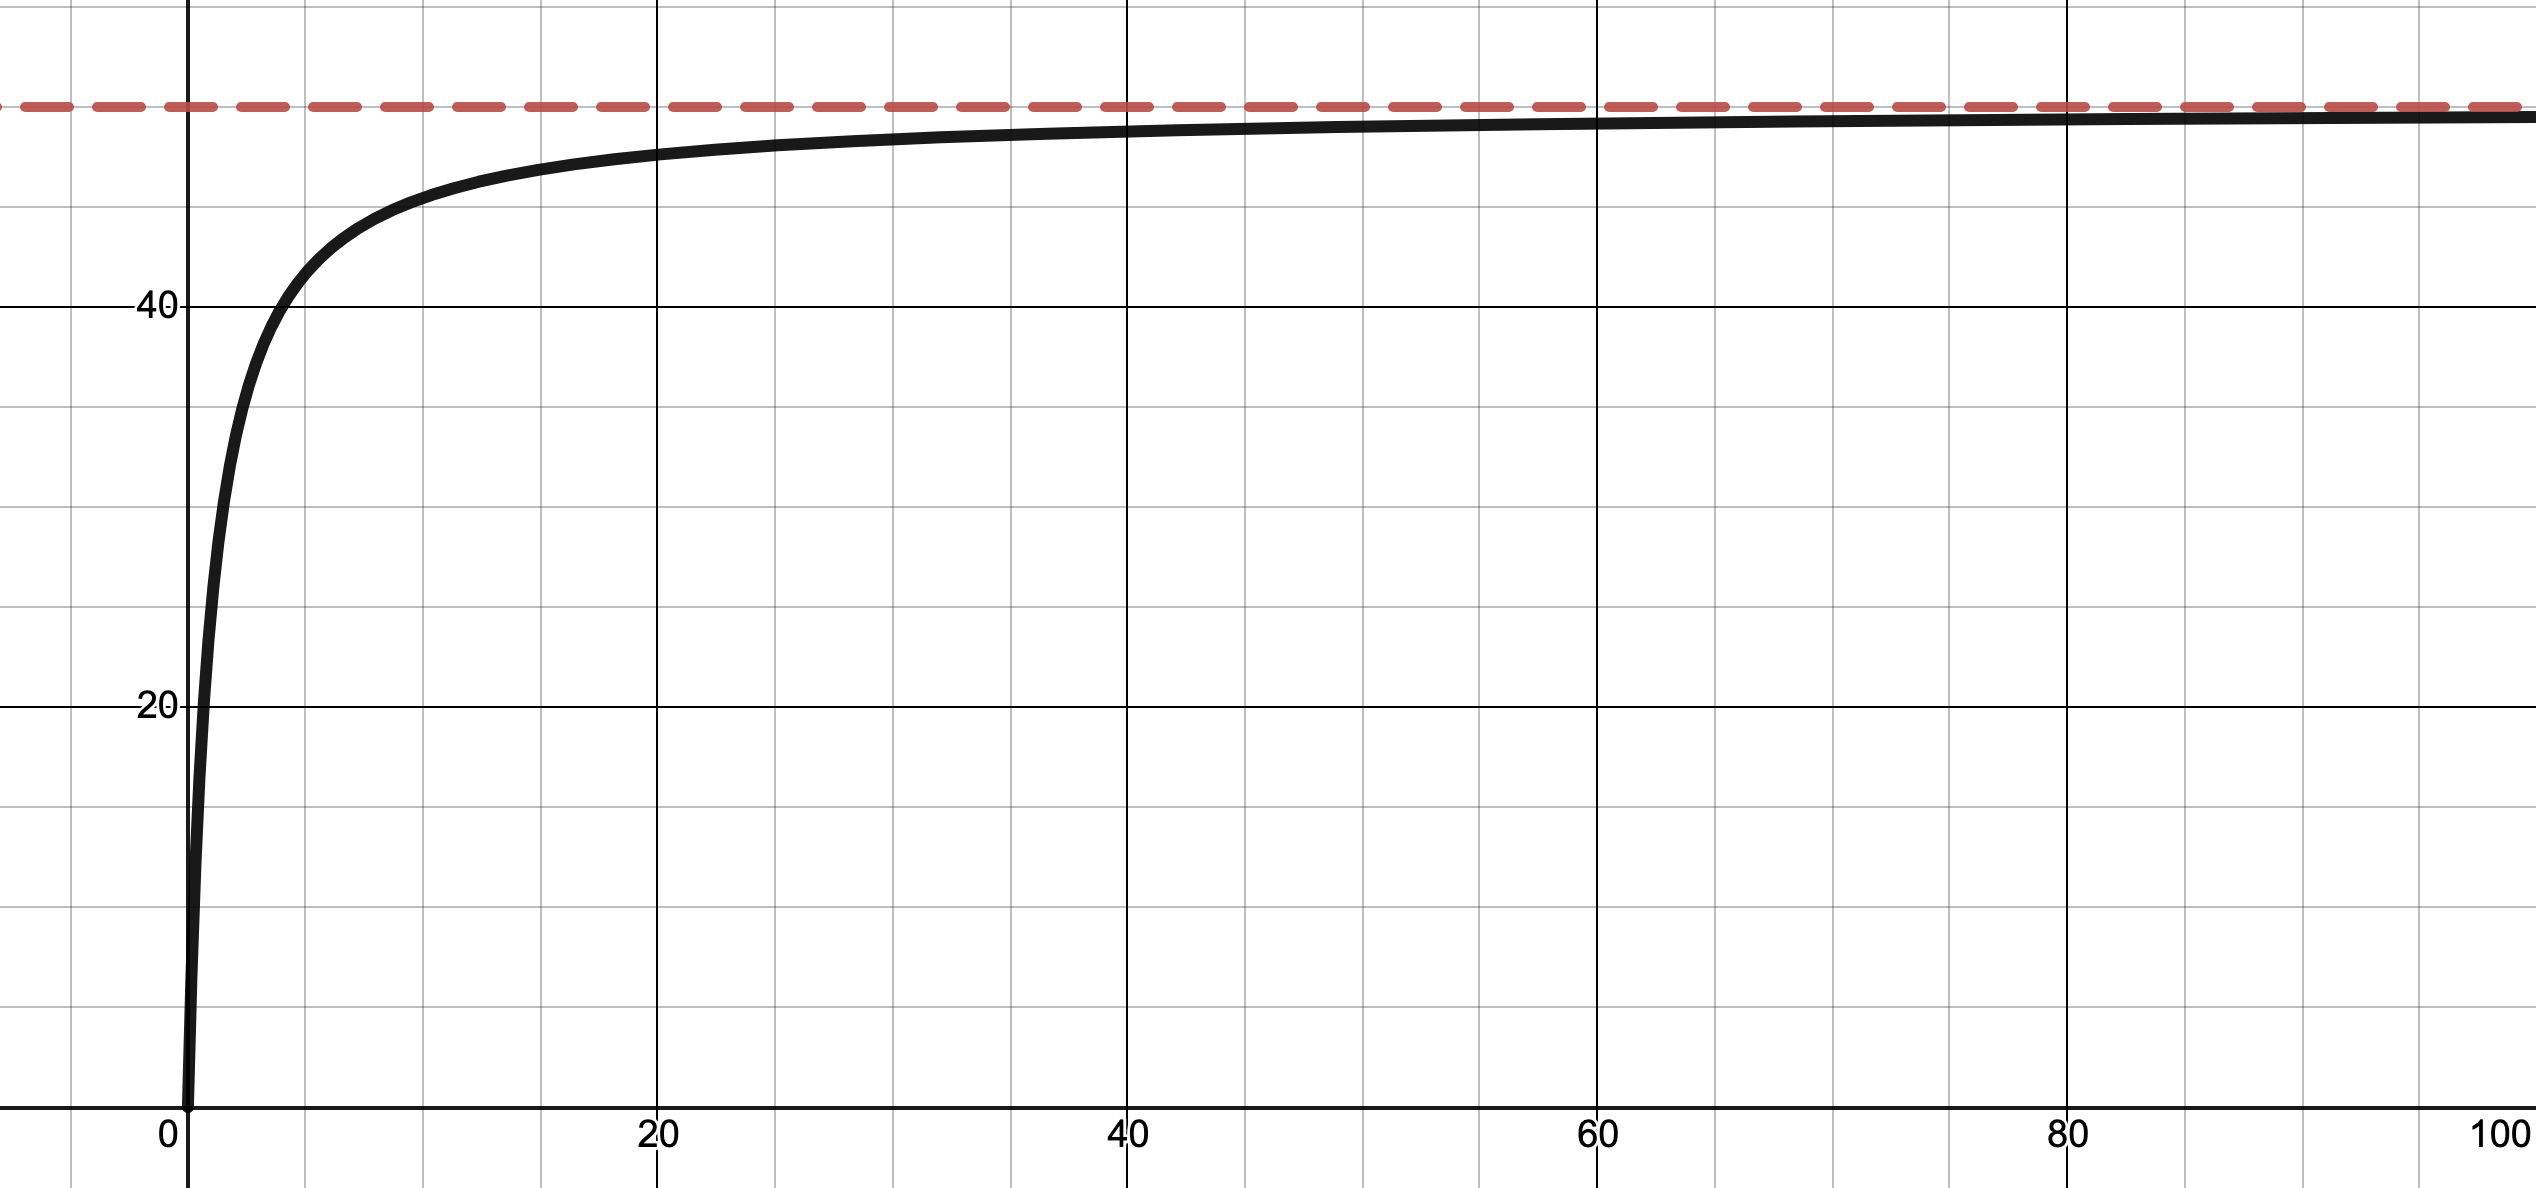
\includegraphics[scale=0.275]{images/productQuotient/11_6c.png}
    \caption{}
    \end{figure}
\newpage


%%%%%%%%%%%%%%%%%%%%%%%%%%%%%%%%%%%%%%%%%%%%%
%%%%%%%%%%%%End Examples%%%%%%%%%%%%%%%%%%
%%%%%%%%%%%%%%%End Topic%%%%%%%%%%%%%%%%%%



%%%%%%%%%%%%%%%End Lesson%%%%%%%%%%%%%%%%%%
\Closesolutionfile{ans}
\Closesolutionfile{ansL}

%%%Short Answers to Examples%%%
%\vspace*{\fill}
\newpage
\subsection*{Short Answers to Examples}
%\vspace{-0.25cm}
%\begin{multicols}{2}
\input{ans10}
%\end{multicols}


